% \documentclass[sigconf]{acmart}
\documentclass[sigconf,review]{acmart}\settopmatter{printfolios=true}

\usepackage{amssymb}
\usepackage{amsthm}
\usepackage{graphicx}
\usepackage{amsmath}
\usepackage{mathptmx}
\usepackage{mathtools}
\usepackage{stmaryrd}
\usepackage{adjustbox}
\usepackage{hyperref}
\usepackage{alltt}
\usepackage{url}
\usepackage{float}
\usepackage{minipage-marginpar}
\usepackage{style/utils}
\usepackage{style/code}
\usepackage{style/proof}
\usepackage{style/keywords}
\usepackage{style/layout}
\usepackage{style/judgements}

% for combinator pictures
\usepackage{tikz}
\usepackage{pgfplots}
\usetikzlibrary{shapes,arrows}

%\setcopyright{none}
\bibliographystyle{ACM-Reference-Format}
% \citestyle{acmauthoryear}

% -----------------------------------------------------------------------------
\begin{document}

\copyrightyear{2017}
\acmYear{2017}
\setcopyright{acmlicensed}
\acmConference{PPDP'17}{October 9--11, 2017}{Namur, Belgium}\acmPrice{15.00}\acmDOI{10.1145/3131851.3131865}
\acmISBN{978-1-4503-5291-8/17/10}

\begin{CCSXML}
<ccs2012>
<concept>
<concept_id>10003752.10003753.10003760</concept_id>
<concept_desc>Theory of computation~Streaming models</concept_desc>
<concept_significance>500</concept_significance>
</concept>
</ccs2012>
\end{CCSXML}


\renewcommand{\textrightarrow}{$\rightarrow$}

\ccsdesc[500]{Theory of computation~Streaming models}


\title{Machine Fusion}
\subtitle{Merging merges, more or less}

\author{Amos Robinson}
\affiliation{Ambiata and UNSW (Australia)}
\email{amosr@cse.unsw.edu.au}

\author{Ben Lippmeier}
\affiliation{Digital Asset and UNSW (Australia)}
\email{benl@ouroborus.net}

\makeatactive
\begin{abstract}
Compilers for stream programs often rely on a fusion transformation to convert the implied dataflow network into low-level iteration based code. Different fusion transformations handle different sorts of networks, with the distinguishing criteria being whether the network may contain splits and joins, and whether the set of fusible operators can be extended. We present the first fusion system that simultaneously satisfies all three of these criteria: networks can contain splits, joins, and new operators can be added to the system without needing to modify the overall fusion transformation.
\end{abstract}

\maketitle

%!TEX root = ../Main.tex
\section{Introduction}

Data flow fusion~\cite{lippmeier2013flow} is a technique to compile a specific class of data flow programs into single, efficient imperative loops. This process of ``compilation'' is equivalent to performing array fusion on a combinator based functional array program, as per related work on stream fusion~\cite{coutts2007streamfusion} and delayed arrays~\cite{keller2010repa}. The key benefits of data flow fusion over this prior work are: 1) it fuses programs that use branching data flows where a produced array is consumed by several consumers, and 2) complete fusion into a single loop is guaranteed for all programs that operate on the same size input data, and contain no fusion-preventing dependencies between operators.

Fusion-preventing dependencies express the fact that some operators simply must wait for others to complete before they can produce their own output. For example, in the following:
\begin{code}
  normalize :: Array Int -> Array Int
  normalize xs = let sum = fold (+) 0 xs
                 in  map (/ sum) xs
\end{code}

If we wish to divide every element of an array by the sum of all elements, then it seems we are forever destined to compute the result using at least two loops: one to determine the sum, and one to divide the elements. The evaluation of @fold@ demands all elements of its source array, and we cannot produce any elements of the result array until we know the value of @sum@. 

However, many programs \emph{do} contain opportunities for fusion, if we only knew which opportunities to take. The following example offers \emph{several} unique, but mutually exclusive approaches to fusion. Figure~\ref{f:normalize2-cluterings} on the next page shows some of the possibilities.
\begin{code}
 normalize2 :: Array Int -> Array Int
 normalize2 xs
  = let sum1 = fold   (+)  0   xs
        gts  = filter (> 0)    xs
        sum2 = fold   (+)  0   gts
        ys1  = map    (/ sum1) xs
        ys2  = map    (/ sum2) xs
    in (ys1, ys2)
\end{code}

In Figure~\ref{f:normalize2-cluterings}, the dotted lines show possible clusterings of operators. Stream fusion implicitly choses the solution on the left as its compilation process cannot fuse a produced array into multiple consumers. The best existing ILP approach will chose the solution on the right as it cannot cluster operators that consume arrays of different lengths. Our system choses the solution in the middle, which is also optimal for this example. 

% NOTE: This set of bullets needs to fit on the first page, without spilling to the second.
Our contributions are as follows:
\begin{itemize}
\item   
We extend prior work by Megiddo~\cite{megiddo1998optimal} and Darte~\cite{darte2002contraction}, with support for length changing operators. Length changing operators can be clustered with the operators that generate their source arrays, and compiled naturally with data-flow fusion (\S\ref{s:ILP}).

\item
We present a simplification to constraint generation that is also applicable to some existing integer linear programming formulations such as Megiddo's,
where constraints between two nodes need not be generated if there exists a fusion-preventing path between the two (\S\ref{s:OptimisedConstraints}).

\item
Our constraint system also encodes a total ordering on the cost of clusterings, expressed using weights on the integer linear program. For example, we encode that memory traffic is more expensive than loop overheads, so given a choice between the two, the memory traffic will be reduced (\S\ref{s:ObjectiveFunction}).

\item
We present benchmarks of our algorithm applied to several common programming patterns, and to several pathological examples.
Our algorithm is complete and yields good results in practice, though if array sizes are unknown, an optimal solution is uncomputable in general. \TODO{ref}
\end{itemize}

The reduction of the clustering problem to integer linear programming was previously described by~\cite{megiddo1998optimal}, though they do not consider length changing operators.


% We must also decide which clustering is the `best' or most optimal. One obvious criterion for this is the minimum number of loops, but there may even be multiple clusterings with the minimum number of loops. In this case, the number of required manifest arrays must also be taken into account. 

% As real programs contain tens or hundreds of individual operators, performing an exhaustive search for an optimal clustering is not feasible, and greedy algorithms tend to produce poor solutions. 


%!TEX root = ../Main.tex

% -----------------------------------------------------------------------------
\section{Processes, Machines, Combinators and Operators}
\label{s:Processes}

A \emph{process} in our system is a simple imperative program with a local heap. A process pulls data from an arbitrary number of input streams and pushes result values to at least one output stream. The process language is an intermediate representation we use when fusing the overall dataflow network. When describing the fusion transform we describe the control flow of the process as a state machine, hence Machine Fusion. 

A \emph{combinator} is a template for a particular process which parameterises it over the particular input and output streams, as well as values of configuration parameters such as the worker function used in a @map@ process. Each process implements a logical \emph{operator} --- so we use ``operator'' when describing the values being computed, but ``process'' and ``machine'' when referring to the implementation. 


% -----------------------------------------------------------------------------
\subsection{Grouping}

The definition of the @group@ combinator which removes consecutive elements from its input stream is given in Fig.~\ref{fig:Process:Group}. We include the concrete code representation and a diagram of the process viewed as a state machine.

The @group@ combinator has two parameters, @sIn1@ and @sOut1@, which bind the input and output streams respectively. The \emph{nu-binders} \mbox{$\nu$ @(f: Bool) (l: Nat)@...} indicate that each time the @group@ combinator is instantiated, fresh names must be given to @f@, @l@ and so on, that do not conflict with other instantiations. 

The body of the combinator is a record that defines the process. The @ins@ field of the record defines the set of input streams and the @outs@ field the set of output streams. The @heap@ field gives the initial values of each of the local variables. The @instrs@ field contains a set of labeled instructions that define the program, while the @label@ field gives the label of the initial instruction. 

%%% AR: Should we explain intuition behind how process works and @f@, @l@, @v@ before detailed instructions?

The initial instruction @(pull sIn1 v A1 [])@ pulls the next element from the stream @sIn1@, writes it into the heap variable @v@ (value), then proceeds to the instruction at label @A1@. The empty list @[]@ after the target label @A1@ can be used to update heap variables, but as we do not need to update anything yet we leave it empty. 

Next, the instruction @(case (f || (l /= v)) A2 [] A3 [])@ checks whether predicate @(f || (l /= v))@ is true; if so it proceeds to the instruction at label @A2@, otherwise it proceeds to @A3@. We use the variable @l@ (last) to track the last value read from the stream, and the boolean @f@ (first) for whether this is the first element.

When the predicate is true, the instruction @(push sOut1 v A3 [ l = v, f = F ])@ pushes the value @v@ to the output stream @sOut1@ and proceeds to the instruction at label @A3@, once the heap has been updated to set variable @l@ to @v@ and @f@ to @F@ (False). 

Finally, the instruction @(drop sIn1 A0 [])@ signals that the current element that was pulled from stream @sIn1@ is no longer required, and goes back to the first the instruction at @A0@. This @drop@ instruction is used to coordinate concurrent processes when performing fusion. The next element of a stream may only be pulled after all consumers have pulled and then and dropped the current element.

Overall, the @f@ variable tracks whether we are dealing with the first value from the stream, @l@ holds the last value pulled from the stream (or 0 if none have been read yet), and @v@ holds the current value pulled from the stream. The process emits the first value pulled from the stream and every value that is different from the last one that was pulled. For example, when executed on the input stream $[1, 2, 2, 3]$, the process will produce the output $[1, 2, 3]$.

\begin{figure}

\begin{center}
\begin{alltt}
           group 
             = \(\lambda\) (sIn1: Stream Nat) (sOut1: Stream Nat). 
               \(\nu\) (f: Bool) (l: Nat) (v: Nat) (A0..A3: Label).
\end{alltt}
\begin{code}
               process
               { ins:    { sIn1  }
               , outs:   { sOut1 }
               , heap:   { f = T, l = 0, v = 0 }
               , label:  A0
               , instrs: { A0 = pull sIn1 v          A1 []
                         , A1 = case (f || (l /= v)) A2 []  A3 []
                         , A2 = push sOut1 v         A3 [ l = v, f = F ]
                         , A3 = drop sIn1            A0 [] } }
\end{code}
\end{center}
\vspace{1em}
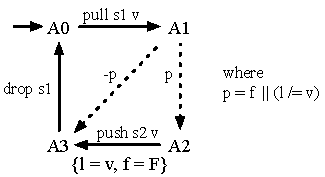
\includegraphics[scale=1.1]{figures/state-group.pdf}
\caption{The group combinator}
\label{fig:Process:Group}
\end{figure}


% -----------------------------------------------------------------------------
\subsection{Merging}
\begin{figure}
\begin{alltt}
               merge
                 = \(\lambda\) (sIn1: Stream Nat) (sIn2: Stream Nat) (sOut2: Stream Nat). 
                   \(\nu\) (x1: Nat) (x2: Nat) (B0..E2: Label).
\end{alltt}
\begin{code}
                   process
                   { ins:    { sM1, sM2 }
                   , outs:   { sM3 }
                   , heap:   { x1 = 0, x2 = 0 }
                   , label:  B0
                   , instrs: { B0 = pull sIn1  x1   B1 []
                             , B1 = pull sIn2  x2   C0 []
                             , C0 = case (x1 < x2)  D0 []  E0 []
                             , D0 = push sOut2 x1   D1 []
                             , D1 = drop sIn1       D2 []
                             , D2 = pull sIn1  x1   C0 []
                             , E0 = push sOut2 x2   E1 []
                             , E1 = drop sIn2       E2 []
                             , E2 = pull sIn2 x2    C0 [] } }
\end{code}

\medskip
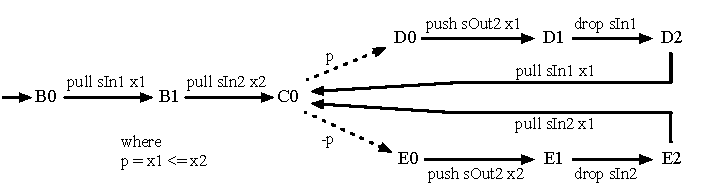
\includegraphics[scale=1.1]{figures/state-merge.pdf}
\caption{The merge combinator}
\label{fig:Process:Merge}
\end{figure}

The definition of the @merge@ combinator, which merges two input streams, is given in Fig.~\ref{fig:Process:Merge}. The combinator binds the two input streams to @sIn1@ and @sIn2@, while the output stream is @sOut2@. The two heap variables @x1@ and @x2@ are used to store the last values read from each input stream. The process starts by pulling from each of the input streams. It then compares the two pulled values, and pushes the smaller of the values to the output stream. The process then drops the stream which yielded the the smaller value, then pulls from the same stream so that it can perform the comparison again.

As this the @merge@ process merges infinite streams, if we execute it with a finite input prefix, it will arrive at an intermediate state that may not yet have pushed all available output. For example, if we execute the process with the input streams $[1, 4]$ and $[2, 3, 100]$ then the values $[1, 2, 3, 4]$ will be pushed to the output. After pushing the last value $4$, the process will block at instruction @E2@, waiting for the next value to become available from @sIn2@. We discuss how to handle finite streams later in ~\S\ref{s:Finite}.


% -----------------------------------------------------------------------------
\subsection{Fusion}

Our fusion algorithm takes two process state machines and produces a new one that computes the outputs of both. For example, suppose we need a single machine that computes the outputs of the first two combinators of our @uniquesUnion@ example back in \S\ref{s:Introduction}. The result will be a machine that computes the result of both the @group@ and @merge@ as if they were executed concurrently, where the first input stream of the @merge@ is the same as the input stream of the @group@. For ease of comparison we will assume the parameters in each combinator are instantiated by arguments with the same names.


% -----------------------------------------------------------------------------
\subsubsection{Fusing Pulls}
\label{s:Fusion:FusingPulls}

The algorithm proceeds by considering pairs of states: one in each of the machines to be fused. Both the @group@ machine and the @merge@ machine pull from the same stream as their initial instruction, so we have the situation shown in Fig.~\ref{fig:Fusion:Pulls}. The @group@ machine needs to transition from label @A0@ to label @A1@, and the @merge@ machine from @B0@ to @B1@. In the result machine we produce three new instructions that transition between four result states, @F0@ to @F3@.
Each of the result states represents a combination of two original states, one from each of the input machines. For example, the first result state @F0@ represents a combination of the @group@ machine being in its initial state @A0@ and the @merge@ machine being in its own initial state @B0@. 

We also associate each of the result states with information describing whether or not each machine has already pulled a value from each input stream. For the @F0@ case shown in Fig.~\ref{fig:Fusion:Pulls} we have ((A0, \{sIn1 = none\}), (B0, \{sIn1 = none, sIn2 = none\})). The result state @F0@ represents a combination of the two input states @A0@ and @B0@. As both @A0@ and @B0@ are the initial states of their respective machines, those machines have not yet pulled any values from their two input streams, so both `sIn1' and `sIn2' map to `none'.

From the joint state @F0@, both of the input machines then need to pull from stream @sIn1@, the @group@ machine storing the value in a variable @v@ and the @merge@ machine storing it in @x1@. In the result machine this is managed by first storing the pulled value in a fresh buffer variable @b1@, and then using later instructions to copy the value into the original variables @v@ and @x1@. For this we attach updates to a @jump@ instruction, which otherwise transitions between states without affecting any of the input or output streams.

Finally, note that in the result states @F0@ through @F3@ the state of the input streams transition from `none', to `pending' then to `have'. The `none' state means that we have not yet pulled a value from the associated stream. The `pending' state means we have pulled a value into the stream buffer variable (@b1@ in this case). The `have' state means that we have copied the pulled value from the stream buffer variable into the local variable used by each machine. In Fig.~\ref{fig:Fusion:Pulls},  `sIn1' is set to `have' for the first machine in @F2@ after we have set `v = b1', while `sIn1' is set to `have' for the second machine in @F3@ after we have set `x1 = b1'. 


\begin{figure}
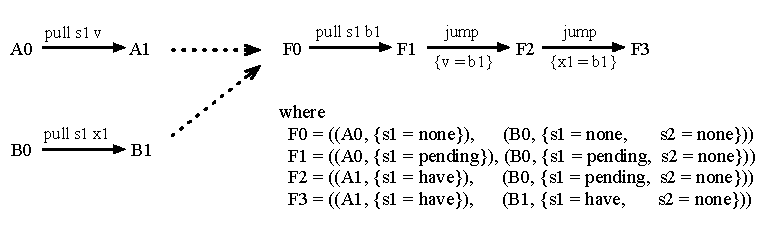
\includegraphics[scale=1.1]{figures/fuse-pull-pull.pdf}
\caption{Fusing pull instructions}
\label{fig:Fusion:Pulls}
\end{figure}


% -----------------------------------------------------------------------------
\subsubsection{Fusing Cases}
\begin{figure}
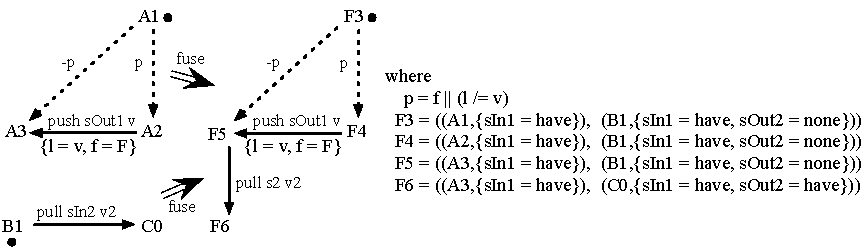
\includegraphics[scale=1.1]{figures/fuse-case-pull.pdf}
\caption{Fusing case instructions}
\label{fig:Fusion:Case}
\end{figure}

Once the result machine has arrived in the joint state @F3@, this is equivalent to the two input machines arriving in states @A1@ and @B1@ respectively. The left of Fig.~\ref{fig:Fusion:Case} shows the next few transitions of these machines. From state @A1@, the @group@ machine needs to perform a @case@ branch to determine whether to push the current value it has from its input stream @sIn1@ to its output stream @sOut1@, or to just move on to the next value from its input. From state @B1@, the @merge@ machine needs to pull a value from its second input stream @sIn2@. In the result machine, @F3@ performs the case analysis from @A1@, moving to either @A2@ or @A3@, corresponding to @F4@ and @F5@ respectively. At @F4@, the push at @A2@ is executed and moves to @A3@, corresponding to @F5@.

Finally, at @F5@ the @merge@ machine pulls from @sIn2@, moving from @B1@ to @C0@.
Because the stream @sIn2@ is only pulled from by the @merge@ machine, no coordination is required between @merge@ and @group@ for this pull.

Note that we could construct the fused result machine in several ways. One option is to perform the case branch first and then pull from @sIn2@, another is to pull from @sIn2@ first and then perform the branch. By construction, the predicate used in the branch refers only to variables local to the @group@ machine, and the pull instruction from @B1@ stores its result in a variable local to the @merge@ machine. As the set of variables does not overlap, either ordering is correct. For this example we choose to perform the branch first, though will discuss the ramifications of this choice further in \S\ref{s:FusionOrder}. 


% -----------------------------------------------------------------------------
\subsection{Fused Result}

Fig.~\ref{fig:Process:Fused} shows the end result of fusing @group@ and @merge@ together. There are other rules for handling different combinations of instructions, but we defer the details to \S\ref{s:Fusion}. The result process has two inputs, @sIn1@ and @sIn2@, which correspond to the original input streams. It also has two outputs, @sOut1@ which is the @group@ processes output stream, while @sOut2@ is the @merge@ processes output stream. 

Overall, our fusion algorithm has taken two separate processes that we once imagined to be running concurrently, and has produced a single sequental result process that implements both. We have chosen a \emph{specific sequential order} in which to interleave instructions that implement both original processes. As with the Flow Fusion system of \citet{lippmeier2013data} we have performed the job of a concurrent scheduler at compile time. However, in contrast to Flow Fusion and similar systems, we do not need to organize statements into a fixed \emph{loop anatomy}, we simply merge them as they are. This allows us to implement a wider range of processes, including ones with nested loops that work on segmented streams, which we discuss further in \S\ref{s:FutureWork}. 

To complete the implementation of our example from \S\ref{s:Introduction} we would now proceed to fuse the process from the final line (also a @group@) into this new result process. The order in which processes are fused together does matter, as does the order in which the instructions are emitted --- we discuss both points further in \S\ref{s:Evaluation}.

Finally, although the result process has a single shared heap, the bindings are guaranteed not to interfere. When we instantiated combinators to create the original processes we introduced fresh names at that point. The stream buffer variables we aditionally introduced for coordination were freshly created during fusion.

%%% AR: would like to highlight which machine is performing the current instruction, eg bolding "A0" when it's group moving from A0 to A1
\begin{figure}
\definecolor{groupc}{HTML}{308030}
\definecolor{mergec}{HTML}{800000}
\definecolor{sharec}{HTML}{000080}

\newcommand\tctt[2]{\textcolor{#1}{\tt{#2}}}
\begin{alltt}
process
\string{ ins:    \string{ \tctt{sharec}{sIn1},  \tctt{mergec}{sIn2} \string}
, outs:   \string{ \tctt{groupc}{sOut1}, \tctt{mergec}{sOut2} \string}
, heap:   \string{ \tctt{groupc}{f = T, l = 0, v = 0}, \tctt{mergec}{x1 = 0, x2 = 0}, \tctt{sharec}{b1 = 0} \string}
, label:  \tctt{sharec}{F0}
\end{alltt}

\newcommand\annot[5]{
  \tiny ((#1,   \> \tiny \{sIn1 =      #2\}), 
                \> \tiny (#3, \> \tiny \{sIn1 =      #4, \> \tiny sIn2 =      #5\}))
}

\newcommand\icase[7]{
 \tt{#1} \> \tt{= #2} \> \tt{#3} \> \tt{[ #4 ]} \> \tt{#5} \> \tt{[ #6 ]} \> \tiny #1 \> \tiny = #7
}
\newcommand\instr[5]{
 \tt{#1}\>\tt{= #2} \> \tt{#3} \> \tt{[ #4 ]} \> \> \> \tiny #1 \> \tiny = #5
}

\begin{tabbing}
@  @ \=
@, F17@  \= = @case (f || (l /= v)) @
         \= @F17@ \= @[ ]     @ \= @F17@ \= @[ ]@
@   @ \= \tiny @   @F17 \= \tiny = ((A0, \= \tiny \{sIn1 = pending\}), \= \tiny (B0, \= \tiny \{sIn1 = pending, \= \tiny sIn2 = pending\})) \kill

@, instrs:@

% I have no idea how this works, but you need this particular incantation to colour the whole line in a tabbing environment.
% It's not ideal that the { and , are coloured too, but that can't be helped.
\\[0pt \color{sharec}]
\> @{@
\instr{F0}{pull sIn1 b1}{F1}{}
      {\annot{A0}{none}{B0}{none}{none}}

\\[0pt \color{groupc}]
\> @,@
\instr{F1}{jump}{F2}{v  = b1}
      {\annot{A0}{pending}{B0}{pending}{none}}

\\[0pt \color{mergec}]
\> @,@
\instr{F2}{jump}{F3}{x1 = b1}
      {\annot{A1}{have}{B0}{pending}{none}}

\\[0pt \color{groupc}]
\> @,@
\icase{F3}{case (f || (l /= v))}{F4}{}{F5}{}
      {\annot{A1}{have}{B1}{have}{none}}

\\[0pt \color{groupc}]
\> @,@
\instr{F4}{push sOut1 v}{F5}{l = v, f = F}
      {\annot{A2}{have}{B1}{have}{none}}

\\[0pt \color{groupc}]
\> @,@
\instr{F5}{jump}{F6}{}
      {\annot{A3}{have}{B1}{have}{none}}

\\[0pt \color{mergec}]
\> @,@
\instr{F6}{pull sIn2 x2}{F7}{}
      {\annot{A0}{none}{B1}{have}{none}}

\\
\\[0pt \color{mergec}]
\> @,@
\icase{F7}{case (x1 < x2)}{F8}{}{F16}{}
      {\annot{A0}{none}{C0}{have}{have}}

\\
\\[0pt \color{mergec}]
\> @,@
\instr{F8}{push sOut2 x1}{F9}{}
      {\annot{A0}{none}{D0}{have}{have}}

\\[0pt \color{mergec}]
\> @,@
\instr{F9}{drop sIn1}{F10}{}
      {\annot{A0}{none}{D1}{none}{have}}

\\[0pt \color{sharec}]
\> @,@
\instr{F10}{pull sIn1 b1}{F11}{}
      {\annot{A0}{none}{D2}{none}{have}}

\\[0pt \color{groupc}]
\> @,@
\instr{F11}{jump}{F12}{v = b1}
      {\annot{A0}{pending}{D2}{pending}{have}}

\\[0pt \color{mergec}]
\> @,@
\instr{F12}{jump}{F13}{x1 = b1}
      {\annot{A1}{have}{D2}{pending}{have}}

\\[0pt \color{groupc}]
\> @,@
\icase{F13}{case (f || (l /= v))}{F14}{}{F15}{}
      {\annot{A1}{have}{C0}{have}{have}}

\\[0pt \color{groupc}]
\> @,@
\instr{F14}{push sOut1 v}{F15}{l = v, f = F}
      {\annot{A2}{have}{C0}{have}{have}}

\\[0pt \color{groupc}]
\> @,@
\instr{F15}{jump}{F7}{}
      {\annot{A3}{have}{C0}{have}{have}}

\\

\\[0pt \color{mergec}]
\> @,@
\instr{F16}{push sOut2 x2}{F17}{}
      {\annot{A0}{none}{E0}{have}{have}}

\\[0pt \color{mergec}]
\> @,@
\instr{F17}{drop sIn2}{F18}{}
      {\annot{A0}{none}{E1}{have}{have}}

\\[0pt \color{mergec}]
\> @,@
\instr{F18}{pull sIn2}{F7}{}
      {\annot{A0}{none}{E2}{have}{none}}


\\[0pt \color{black}]
@} }@
\end{tabbing}

\caption{Fusion of \textcolor{groupc}{group} and \textcolor{mergec}{merge}, along with \textcolor{sharec}{shared} instructions}
\label{fig:Process:Fused}
\end{figure}


% -----------------------------------------------------------------------------
% BL: This is too much low level detail at this point, we need more intuition.

% The instructions of @merge@ can be split into four categories, which can be identified in the fused process: labels @B0@-@B2@ perform initialisation, and are mapped to @F0@-@F6@; label @C0@ performs case analysis to find the smaller value and is mapped to @F7@; labels @D0@-@D2@ push the value from the first stream, @s1@, and are mapped to @F8@-@F15@; and labels @E0@-@E2@ push the value from the second stream, @s2@, and are mapped to @F16@-@F18@.

% The @group@ process can also be identified in the fused process: the fused labels @F0@-@F5@ perform the pulling, case analysis and pushing from instructions @A0@-@A2@. These instructions are seen again in @F10@-@F14@, when the @merge@ process is pulling from the @s1@ stream. Thus the @group@ instructions have been duplicated, and are performed once when @merge@ initialises, and again every time @merge@ pulls from the first stream.

% Labels @F5@ and @F14@ correspond to the (@drop s1@) instruction at @A3@ in @group@, but note that they are fused as @jump@ instructions. As @s1@ is shared between the two processes, the element from @s1@ can only be dropped once both processes agree to drop. In the fused labels on the right hand column, the other process still has @s1@ as `pending' or `have', so the element cannot yet be dropped. The actual @drop@ is only performed once both processes are `none', at label @F9@.
 

%!TEX root = ../Main.tex

\clearpage{}
% -----------------------------------------------------------------------------
\section{Process definitions}
%!TEX root = ../Main.tex

\begin{figure}
\begin{minipage}[t]{0.4\textwidth}
\begin{tabbing}
\Instr \TABDEF @MMMM@  \TABSKIP $\Exp$ \TABSKIP $\Exp$ \TABSKIP $\Exp$ \kill

\Exp,~$e$ \> $\to$ \> $x~|~v~|~e~e $ \\
  \> $\enskip|~$ \> $ (e~||~e) ~|~ e+e ~|~ e~@/=@~e ~|~ e < e$ \\
\Value,~$v$ \> $\to$ \> $\mathbb{N}~|~\mathbb{B}~|~(\lambda{}x.~e)$ \\
\Heap,~$\Sigma$ \> $\to$ \> $\cdot~|~\Sigma,~x~=~v$ \\
\\

\Proc \>:=\> @process@ \\
MMMMMM \= M \= \kill
\> \> @ins:   @  $(\Chan ~\mapsto~ \InputState)$ \\
\> \> @outs:  @  $\sgl{\Chan}$ \\
\> \> @heap:  @  \Heap \\
\> \> @label: @  \Label \\
\> \> @instrs:@  $(\Label ~\mapsto~ \Instr)$ \\
\\
\Instr \TABDEF \kill
\InputState \> := \> @none@~$|$~@pending@~\Value~$|$~@have@

\end{tabbing}
\end{minipage}
\begin{minipage}[t]{0.05\textwidth}
\quad
\end{minipage}
\begin{minipage}[t]{0.4\textwidth}
\begin{tabbing}
\Instr \TABDEF @MMMM@  \TABSKIP $\Chan$ \TABSKIP $\Chan$ \TABSKIP $\Exp$ \kill

\Var,~$x$ \> $\to$ \> (value variable) \\
\Chan,~$c$ \> $\to$ \> (channel/stream name) \\
\Label,~$l$ \> $\to$ \> (label name) \\
\\
\\

\Instr
    \> :=\> @pull@  \> \Chan  \> \Var  \> \Next \\
    \TABALT @push@  \> \Chan  \> \Exp  \> \Next \\
    \TABALT @case@  \> \Exp   \> \Next \> \Next \\
    \TABALT @jump@  \>        \>       \> \Next \\
    \TABALT @drop@  \> \Chan  \>       \> \Next \\
\\
\\
\Next \> := \> $\Label~\times~(\Var \mapsto \Exp)$ \\
\end{tabbing}
\end{minipage}
\caption{Process definitions}
\label{fig:Process:Def}
\end{figure}



The grammar for process definitions is given in Fig.~\ref{fig:Process:Def}. Variables, Channels and Labels are specified by unique names. We refer to the \emph{endpoint} of a stream as a channel. A particular stream may flow into the input channels of several different processes, but can only be produced by a single output channel. For values and expressions we use an untyped lambda calculus with a few primitives chosen to facilitate the examples. The `$||$' operator is boolean-or, `+' addition, `/=' not-equal, and `$<$' less-then.

A $\Proc$ is a record with five fields: the @ins@ field specifies the input channels; the @outs@ field the output channels; the @heap@ field the process-local heap; the @label@ field the label of the currently being executed instruction, and the @instrs@ a map of labels to instructions. We use the same record when specifying both the definition of a particular process, as well as when giving the evaluation semantics. When specifying a process the @label@ field gives the entry-point to the process code, though during evaluation it is the label of the instruction currently being executed. Likewise, when specifying a process we usually only list channel names in the @ins@ field, though during evaluation they are also paired with their current $\InputState$. If an $\InputState$ is not specified we assume it is `none'.

In the grammar of Fig.~\ref{fig:Process:Def} the $\InputState$ has three options: @none@, which means no value is currently stored in the associated stream buffer variable, $(@pending@~\Value)$ which gives the current value in the stream buffer variable and indicates that it has not yet been copied into a process-local variable, and @have@ which means the pending value has been copied into a process-local variable. The $\Value$ attached to the @pending@ state is used when specifying the evaluation semantics of processes. During fusion, the $\Value$ itself will not be known, but we can still reason statically that a process must be in the @pending@ state. We will use a different version of $\InputState$ in \S\ref{s:Fusion} when we define the fusion algorithm.

The @instrs@ field of the $\Proc$ maps labels to instructions. The possible instructions are: @pull@, which pulls the next value from a channel into a given heap variable; @push@, which pushes the value of an expression to an output channel; @case@ which branches depending on the result of a boolean expression; @jump@ which causes control to move to a new instruction, and @drop@ which indicates that the current value pulled from a channel is no longer needed. 

All instructions include a $\Next$ field which is a pair of the label of the next instruction to execute, as well as a list of $\Var \times \Exp$ bindings used to update the heap. The list of update bindings is attached directly to instructions to make the fusion algorithm easier to specify, in contrast to a presentation with a separate @update@ instruction. 

As with Kahn processes~\cite{kahn1976coroutines}, pulling from a channel is blocking. Unlike Kahn processes, pushing to a channel can also block. Each consumer has a single element buffer, which is the stream buffer variable, and pushing can only succeed when that buffer is empty.

When lowering process code to a target language, such as C, LLVM, or some sort of assembly code, we can safely ignore the @drop@ instructions. The @drop@ instructions are used to help control how processes being fused should be synchronized, but do not affect the execution of a single process. We will discuss @drop@s further in \S\ref{s:Optimisation}.


% -----------------------------------------------------------------------------
\subsection{Execution}
\label{s:Process:Eval}


Execution of process networks consists of three aspects:

\begin{enumerate}
\item \emph{Injection}, which attempts to provide a single value gained from a stream to a process, or a set of processes. Each individual process only needs to accept the value when it is ready for it, and injection of a value into a set of processes succeeds only when they \emph{all} accept it.

\item \emph{Shaking}, which advances a single process from one instruction to another. Shaking a set of processes succeeds when \emph{any} of the processes in the set can advance.

\item \emph{Feeding}, which manages communication between separate processes in the network. Feeding alternates between Injecting and Shaking. When a process pushes a value to an output channel we attempt to inject this value into all processes that have that same channel as an input. If they all accept it then we then advance their programs as far as they will go, which may cause more values to be pushed to output channels, and so on.

\end{enumerate}

Evaluation of a process network is non-deterministic. At any moment several processes may be able to take a step, while others are blocked trying to pull or push to their channels. However, because each process itself is deterministic, and uses blocking reads, the sequence of values pushed to each stream is deterministic, as per Kahn process networks. 

Importantly, it is the order in which values are \emph{pushed to each particular output channel} which is deterministic, whereas the order in which different processes execute their instructions, is not. When we fuse two processes together we exploit this fact by choosing one particular instruction ordering that enables the process network to advance without requiring unbounded buffering.

Each output channel may be pushed to by a single process only, so in a sense each output channel is ``owned'' by a single process. The only intra-process communication is via channels and streams. Our model is ``pure data flow'' (or perhaps ``functional data flow'') as there are no side-channels between the processes. This is in contrast to systems such as StreamIt~\cite{thies2002streamit}, where the processes are also able to send asynchronous messages to each other, in addition to the formal input and output streams.



% -----------------------------------------------------------------------------
\subsubsection{Injection}
Fig.~\ref{fig:Process:Eval:Inject} gives the rules for injecting values into processes. The statement $(\ProcInject{p}{v}{c}{p'})$ reads ``given process $p$, injecting value $v$ into channel $c$ yields a new process $p'$''. The @injects@ form is similar, but operates on sets of processes rather than a single one.

Rule (InjectValue) injects of a single value into a single process. The value is stored as a (@pending@~ v) binding in the $\InputState$ for the associated channel of the process. The $\InputState$ acts as a single element buffer, and must be empty (set to @none@) for the injection to succeed.

Rule (InjectIgnore) allows processes that do not use a particular named channel to ignore values injected into that channel.

Rule (InjectMany) attempts to inject a single value into a set of processes. We use the single process judgment form to inject the value into all processes in the set, which must succeed for all of the. Once a value has been injected into all consuming processes that require it, it is then safe for a producing process to discard it.

%!TEX root = ../Main.tex

\begin{figure*}
\begin{minipage}[t]{1\textwidth}

$$
\arrLR{
  \boxed{\ProcInject{\Proc}{\Value}{\Chan}{\Proc}}
}{
  \boxed{\ProcsInject{\sgl{\Proc}}{\Value}{\Chan}{\sgl{\Proc}}}
}
$$

$$
\ruleIN{
  p[@ins@][c] = @none@
}{
  \ProcInject{p}{v}{c}{p~[@ins@ \mapsto (p[@ins@][c \mapsto @pending@~v]) ] }
}{InjectValue}
$$

$$
\ruleIN{
  c \not\in p[@ins@]
}{
  \ProcInject{p}{v}{c}{p}
}{InjectIgnore}
%
\quad
%
\ruleIN{
  \{~ \ProcInject{p_i}{v}{c}{p'_i} ~\}^i
}{
  \ProcsInject{\sgl{p_i}^i}{v}{c}{\sgl{p'_i}^i}
}{InjectMany}
$$

\end{minipage}
\caption{Injection of values into input channels}
\label{fig:Process:Eval:Inject}
\end{figure*}



%!TEX root = ../Main.tex

\begin{figure}

$$
\arrLR{
  \boxed{\ProcInject{\Proc}{\Chan}{\Value}{\Proc}}
}{
  \boxed{\ProcsInject{\sgl{\Proc}}{\Chan}{\Value}{\sgl{\Proc}}}
}
$$

$$
\ruleIN{
  (@ins@~ p)[c] = @none@
}{
  \ProcInject{p}{c}{v}{p~\{@ins@ = (@ins@~p)[c \mapsto @pending@~v] \} }
}{InjectValue}
%
\ruleIN{
  c \not\in @ins@~p
}{
  \ProcInject{p}{c}{v}{p}
}{InjectIgnore}
$$

$$
\ruleIN{
  \{~ \ProcInject{p_i}{c}{v}{p'_i} ~\}^i
}{
  \ProcsInject{\sgl{p_i}}{c}{v}{\sgl{p'_i}}
}{ProcessesInject}
$$

\caption{Injection of values into input channels}
\label{fig:Process:Eval:Inject}
\end{figure}


\begin{figure}

$$
\alpha~@:=@~ \Push~\Chan~\Value ~|~ \tau
$$

$$
  \boxed{
    \ProcBlockShake
      {\Instr}{\MapType{\Chan}{\InputState}}{\Sigma}
      {\alpha}
      {\Label}{\MapType{\Chan}{\InputState}}{\MapType{\Var}{\Exp}}
  }
$$


$$
\ruleIN{
  c=@pending@~v \in i
}{
  \ProcBlockShake{@pull@~c~x~(l,u)}{i}{\Sigma}{\tau}{l}{\HeapUpdateOne{c}{@have@}{i}}{u,~x = v}
}{Pull}
\ruleIN{
  c=@have@ \in i
}{
  \ProcBlockShake{@drop@~c~(l,u)}{i}{\Sigma}{\tau}{l}{\HeapUpdateOne{c}{@none@}{i}}{u}
}{Drop}
$$

$$
\ruleIN{
  \ExpEval{\Sigma}{e}{v}
}{
  \ProcBlockShake{@push@~c~e~(l,u)}{i}{\Sigma}{\Push~c~v}{l}{i}{u}
}{Push}
\ruleIN{
}{
  \ProcBlockShake{@jump@~(l,u)}{i}{\Sigma}{\tau}{l}{i}{u}
}{Jump}
$$

$$
\ruleIN{
  \ExpEval{\Sigma}{e}{@true@}
}{
  \ProcBlockShake{@case@~e~(l_t,u_t)~(l_f,u_f)}{i}{\Sigma}{\tau}{l_t}{i}{u_t}
}{CaseT}
\ruleIN{
  \ExpEval{\Sigma}{e}{@false@}
}{
  \ProcBlockShake{@case@~e~(l_t,u_t)~(l_f,u_f)}{i}{\Sigma}{\tau}{l_f}{i}{u_f}
}{CaseF}
$$

$$
  \boxed{\ProcShake{\Proc}{\alpha}{\Proc}}
  \quad
  \boxed{\ProcsShake{\sgl{\Proc}}{\alpha}{\sgl{\Proc}}}
$$

$$
@let@~@instr@~p~=~@instrs@~p~(@label@~p)
$$
$$
\ruleIN{
  \ProcBlockShake
    {@instr@~p} {@ins@~p}{@heap@~p}
    {\alpha}
    {l}{i}{u}
  \quad
    \ExpEval{@heap@~p}{u}{\Sigma}
}{
  \ProcShake{p}{\alpha}{p~\sgl{@label@~=~l,~@heap@~=~(\HeapUpdates{\Sigma}{@heap@~p}),~@ins@~=~i}}
}{Shake}
$$




$$
\ruleIN{
  \ProcShake{p_i}{\tau}{p'_i}
}{
  \ProcsShake{
    \sgl{p_0 \ldots p_i \ldots p_n}
  }{\tau}{
    \sgl{p_0 \ldots p'_i \ldots p_n}
  }
}{ProcessesInternal}
$$

$$
\ruleIN{
  \ProcShake{p_i}{\Push~c~v}{p'_i}
  \quad
  \forall j~|~j \neq i.~
  \ProcInject{p_j}{c}{v}{p'_j}
}{
  \ProcsShake{
    \sgl{p_0 \ldots p_i \ldots p_n}
  }{\Push~c~v}{
    \sgl{p'_0 \ldots p'_i \ldots p'_n}
  }
}{ProcessesPush}
$$


\caption{Evaluation: shaking allows proceses to take a step from one label to another as well as produce an output message.
If the message is a push, the value is injected to all other processes in the network; otherwise it is an internal step.}
\label{fig:Process:Eval:Shake}
\end{figure}


%!TEX root = ../Main.tex

\begin{figure}

$$
  \boxed{
    \ProcsFeed
      {\MapType{\Chan}{[\Value]}}
      {\sgl{\Proc}}
      {\MapType{\Chan}{[\Value]}}
      {\sgl{\Proc}}
  }
$$

\newcommand\vs {\ti{vs}}
\newcommand\accs {\ti{accs}}
\newcommand\network {\ti{ps}}

$$
\ruleIN{
  \forall c \in \accs.~
  \accs~c~=~[]
}{
  \ProcsFeed
    {\accs}
    {\network}
    {\accs}
    {\network}
}{FeedStart}
%
\ruleIN{
  \ProcsFeed
    {\accs}
    {\network}
    {\accs'}
    {\network'}
\quad
  \ProcsShake
    {\network'}
    {\tau}
    {\network''}
}{
  \ProcsFeed
    {\accs}
    {\network}
    {\accs'}
    {\network''}
}{FeedInternal}
$$

$$
\ruleIN{
  \ProcsFeed
    {\accs}
    {\network}
    {\accs'}
    {\network'}
\quad
  \ProcsShake
    {\network'}
    {\Push~c~v}
    {\network''}
}{
  \ProcsFeed
    {\accs}
    {\network}
    {c=\accs'~c \listappend [v], \accs'}
    {\network''}
}{FeedPush}
$$

$$
\ruleIN{
  (\forall p \in \network.~c \not\in @outs@~p)
\quad
  \ProcsFeed
    {c=\vs, \accs}
    {\network}
    {\accs'}
    {\network'}
\quad
  \ProcsInject
    {\network'}
    {c}{v}
    {\network''}
}{
  \ProcsFeed
    {c=\vs \listappend [v], \accs}
    {\network}
    {c=\vs \listappend [v], \accs'}
    {\network''}
}{FeedExternal}
$$


\caption{Process evaluation: feeding processes from external streams and collecting outputs}
\label{fig:Process:Eval:Feed}
\end{figure}



% -----------------------------------------------------------------------------
\subsubsection{Shaking}
Fig.~\ref{fig:Process:Eval:Shake} gives the rules for advancing a single process. The first set of rules handle specific instructions. The statement $(\ProcBlockShake{i}{is}{\Sigma}{\alpha}{l}{is'}{us})$ reads ``instruction $i$, given channel states $is$ and the heap $\Sigma$, passes control to instruction at label $l$ and yields new channel states $is$, heap update expressions $us'$, and performs an output action $\alpha$.'' An output action $\alpha$ is a list of messages of the form $(\Push~\Chan~\Value)$, which encode the values a process pushes to its output channels. We write ~$\cdot$~ for an empty action. 

\eject{}
Rule (Pull) takes the @pending@ value $v$ from the channel state and produces a heap update that will copy this value into the variable $x$ named in the @pull@ instruction. We use the syntax $us \rhd x=v$ to mean that the list of updates $us$ is extended with the new binding $x=v$. In the result channel states, the state of the channel $c$ that was pulled from is set to @have@, to indicate the value has been copied.

Rule (Push) evaluates the expression $e$ under heap $\Sigma$ to a value $v$, and produces a corresponding action which carries this value. The judgment $(\Sigma \vdash e \Downarrow v)$ expresses standard simply typed lambda calculus reduction using the heap $\Sigma$ for the values of free variables. As this evaluation is completely standard we omit it to save space.

Rule (Drop) changes the input buffer state from @have@ to @none@. A drop can only be executed after pull has set the input buffer to @have@. 

Rule (Jump) simply produces a new label and update expressions and rules (CaseT) and (CaseF) evaluate the scrutinee $e$ and jump to the appropriate label.

The statement $\ProcShake{p}{\alpha}{p'}$ reads ``process $p$ advances to new process $p'$, yielding action $\alpha$''. Rule (Shake) advances a whole process. We lookup the current instruction pointed to by the processes @label@ and pass it, along with the current channel states and heap to the previous single-instruction judgment. The update expressions @us@ that the single-instruction judgment yields are first reduced to values before updating the heap. The update expressions themselves are all pure, so the evaluation can safely be done in parallel (or in arbitrary order).


% -----------------------------------------------------------------------------
\subsubsection{Feeding}
Fig.~\ref{fig:Process:Eval:Feed} gives the rules for collecting the output actions and feeding output values to other processes. The first set of rules concerns feeding values to other processes within the same process network, while the second exchanges input and output values with the environment the process network is running in.

\eject{}
The statement $\ProcShake{ps}{\alpha}{ps'}$ reads ``the processes group $ps$ advances to the new process group $ps'$ yielding output action $\alpha$. A process ``group'' is just a set of processes. 

Rule (ProcessInternal) allows an arbitrary process in the group to advance to a new state at any time, provided it does not produce an output action. This allows processes to perform internal computation, without needing to synchronize with the rest of the group.

Rule (ProcessPush) allows an arbitrary process in the group to advance to a new state, while producing an output action (@push@ c v). For this to happen it must be possible to inject the output value @v@ into any processes that has channel @c@ as one of its inputs. As all consuming processes must accept the output value at the time it is created, there is no need to buffer it further in the producing process. When any process in the group produces an output action then we take that as the action of the whole group, as it might also need to be sent to the environment. 

\smallskip
The statement $\ProcsFeed{cvs}{ps}{cvs'}{ps'}$ reads ``with channel values $cvs$, process group $ps$ takes a step and produces new channel values $cvs'$ and group $ps'$''. The channel values $cvs$ map channel names to a list of values. For input channels of the overall group, we initialize the map to contain a list of input values for each channel. For output channels of the overall group, values pushed to those channels are also collected in the same channel map. In a concrete implementation the input and output values would be transported over some IO device, but the simplified semantics here is sufficient to describe the abstract behavior of our system.

Rule (FeedInternal) allows the process group to perform local computation in the context of the channel values. 

Rule (FeedPush) collects an output action produced by a process group and adds it to the list corresponding to the output channel.

Rule (FeedExternal) injects values from the external environment. This rule also has the side condition that values cannot be injected from the environment into output channels that are already owned by some process. This constraint is used during formal proofs of correctness, but would not need to be checked dynamically in a concrete implementation. The topology of the dataflow network does not change at runtime, so it only needs to be checked once, before execution.


% -----------------------------------------------------------------------------
\subsection{Non-deterministic Evaluation Order}

The evaluation rules of Fig. \ref{fig:Process:Eval:Feed} are non-deterministic in several ways. Rule (ProcessInternal) allows any process to perform internal computation at any time, without synchronizing with other processes in the group. More importantly, (ProcessPush) allows any process to perform a push action at any time, provided the other processes in the group are ready to accept the pushed value. Rule (FeedExternal) also allows new values pushed into an input channel from the environment, provided all processes that use that channel are ready to accept the value.

In our system, allowing the evaluation order of processes to be non-deterministic is critical, as it provides freedom to search for a valid ordering that does not require excessive buffering. Consider the following example, where the @alt2@ operator pulls two elements form its first input stream, then two from the second, before pushing all four to its output.
\begin{code}
  alternates : S Nat -> S Nat -> S Nat -> S (Nat, Nat)
  alternates sInA sInB sInC
   = let  s1   = alt2 sInA sInB
          s2   = alt2 sInB sInC
          sOut = zip s1 s2
     in   sOut
\end{code}

Note that the middle stream @sIn2@ is shared, and the result streams from both @alt2@ operators are zipped into tuples. Given the inputs @sInA@ = @[a1,a2]@, @sInB@ = @[b1,b2]@ and @sInC@ = @[c1,c2]@ the output of @zip@ will be @[(a1,b1),(a2,b2),(b1,c1),(b2,c2)]@, assuming @a1,a2,b1,b2@ and so on are values of type @Nat@.

Now, note that the first @alt2@ process pushes values to its output stream @s1@ two at a time, and the second @alt2@ process also pushes values to its own output stream @s2@ two at a time. However, the downstream @zip@ process needs to input one value from @s1@ then one from @s2@, then another from @s1@, then another from @s2@, alternating between the @s1@ and @s2@ streams. This will work, provided we can arrange for the two \emph{separate} @alt2@ processes to push to their separate output streams alternatively. They can still push two values at a time to their own outputs, but the downstream @zip@ process needs receive one from each process alternately. Here is a table of intermediate values to help make the explanation clearer:

\begin{code}
    sInA = [a1, a2, a3, a4, a5 ...]
    sInB = [b1, b2, b3, b4, b5 ...]
    sInC = [c1, c2, c3, c4, c5 ...]

    s1   = alt2 sInA sInB 
         = [a1, a2, b1, b2, a3, a4, b3, b4 ...]

    s2   = alt2 sInB sInC
         = [b1, b2, c1, c2, b3, b4, c3, c4 ...]

    sOut = zip s1 s2
         = [(a1,b1), (a2,b2), (b1,c1), (b2,c2) ...]
\end{code}

Considering the last line in the above table, note that @zip@ needs to output a tuple of @a1@ and @b1@ together, then @a2@ and @b2@ together, and so on. The implementation of the @zip@ process will attempt to pull the first value @a1@ from stream @s1@, blocking until it gets it, then pull the next value @b1@ from stream @s2@, blocking until it gets it. While @zip@ is blocked waiting for @b1@, the first @alt2@ process cannot yet push @a2@. The evaluation order of the overall process group is constrained by communication patterns of processes in that group.

As we cannot encode all possible evaluation orderings into the definition of the processes themselves, we have defined the evaluation rules to admit many possible orderings. In a direct implementation of concurrent processes using message passing and operating system threads, an actual, working, evaluation order would be discovered dynamically at runtime. In contrast, the role of our fusion transform is to determine one of these working evaluation orders statically. In the fused result process, the instructions will be scheduled so that they run in one of the orders that we would have gotten if the process group was executed dynamically. In doing so, we also eliminate the need to pass messages between processes --- once they are fused we can just copy values between heap locations.


% Although alt2 produces output elems two at a time, the consumer zip need its input elements to arrive alternately. At evaluation time we need the results pushed to sA1 and sA2 in the sA1 sA2 sA1 sA2 order, not sA1 sA1 sA2 sA2. Writing the rules nondeterministically allows the elaborator to discover a usable order, if there is one. This also affects fusion, we don't want to commit to the wrong order too early. We shall see that if we fuse the two alt processes first fusion will not work. We need to start with zip so that the order in which input elems arrive is constrained. 


% Rule (FeedPush) allows the process network to emit a push message. As with (FeedInternal), it first feeds its input accumulator, then allows the resulting network to emit a push message. The pushed value is collected in the accumulator list for that stream.

% Rule (FeedExternal) allows inputs to be injected into the process network.
% For any channel $c$ which is not an output of one of the processes, we take the last value off its list. The recursive feed is evaluated with the last value removed from the accumulators. The last value is then injected into the network, and added back to the result accumulators.

% Rule (FeedStart) applies when all input values have been injected and there are no input values left. In this case, the output values are the same as the input values.

% Evaluation: feeding evaluates a process network on a list of input values and collects the outputs. Feeding alternates between injecting input values and shaking the processes to collect the output messages.

% Note that the result stream and network are not canonical, as an infinite @push@ loop has an infinite number of evaluations.
% The feed form does not ensure that the processes themselves have finished evaluating, only that all input values have been injected.



% -- cuts ---------------------------------------------------------------------
% BL: Discuss this during def of evaluation.

% These input states are used for evaluation to ensure that communication between processes does not require unbounded buffers.

% Claim "functional dataflow" or some such. Each process only updates values in its local heap, the only intra-process communication is via streams. This is unlike StreamIt which can send out-of-band messages between its processes.

% The output streams are in some sense ``owned'' by the process that produces them: while a stream may be consumed by any number of processes, each stream can only appear as the output for one process. This ensures a sort of determinism in the scheduling of multiple processes; if different processes could push to the same stream, the order of values would depend on the scheduled order. A process may, however, produce multiple output streams.

% Each process has its own private heap, therefore the only communication between processes occurs by streams.

% The instructions (@instrs@) are a mapping from label to instruction, and label points to the current instruction. Instructions can pull from a channel, drop an already pulled value, push a value, perform an if/case analysis on a boolean, or perform an internal jump.


% After values have been pulled, they must be disposed of with @drop@: this empties the value from the buffer and allows the producer to push to the channel.

% A process network is a set of multiple processes that can be evaluated concurrently. Any inputs that are not produced as outputs of processes are assumed to be external inputs --- their values will be provided by the environment. Processes form the essence of stream computation, and a single process can be given a straightforward sequential semantics by mapping to an imperative language. By fusing multiple processes into a single one, we are effectively giving a sequential interpretation for concurrent processes.


%!TEX root = ../Main.tex

% -----------------------------------------------------------------------------
\section{Fusion}
\label{s:Fusion}

The core fusion algorithm constructs a static execution schedule for a single pair of processes. To fuse a whole process network we fuse successive pairs of processes until only one remains. 

Fig.~\ref{fig:Fusion:Types} defines some auxiliary grammar used during fusion. We extend the existing $Label$ grammar with an additional alternative, $Label_F \times Label_F$ for the labels in a fused result process. Each $Label_F$ consists of a $Label$ from one of the source processes, paired with a map from $Channel$ to the statically known part of that channel's current $\InputState$. The definition of $Label$ is now recursive. While fusing a whole network, as we fuse pairs of individual processes the labels in the result collect more and more information. Each label of the final, completely fused process encodes the joint state that all the original source processes would be in at that point.

% These new labels $Label_F$ consist of a pair of source labels, as well as the static part of the $\InputState$ of each input channel. 

% If the static $\InputState_F$ is $@pending@_F$, there is a value waiting to be pulled, do not know the actual value. 

We also extend the existing $\Var$ grammar with a (@chan@ $c$) form which represents the buffer variable associated with channel @c@. We only need one buffer variable for each channel, and naming them like this saves us from inventing fresh names in the definition of the fusion rules.
(We used a fresh name back in \S\ref{s:Fusion:FusingPulls} to avoid introducing a new mechanism at that point in the discussion.) 

Still in Fig.~\ref{fig:Fusion:Types}, $\ChanType_2$ classifies how channels are used, and possibly shared, between two processes. Type @in2@ indicates that the two processes @pull@ from the same channel, and these actions must then be coordinated. Type @in1@ indicates that only a single process pulls from the channel. Type @in1out1@ indicates that one process pushes to the channel and the other pulls. Type @out1@ indicates that the channel is pushed to by a single process. Each output channel is uniquely owned and cannot be pushed to by more than one process.

%!TEX root = ../Main.tex

\begin{figure}

\begin{tabbing}
@MMMMMMMMMMMM@   \TABDEF \kill

$\InputState_S$ \> := \> $@none@_S ~|~ @pending@_S ~|~ @have@_S$
%%% AR: reorder to fit dynamic input state order
\\
$\Label_1$ \> := \> $\Label~\times~\MapType{\Chan}{\InputState_S}$ \\
$\Label$   \> := \> $\ldots ~|~\Label_1~\times~\Label_1 ~|~ \ldots$ \\
$\Var$     \> := \> $\ldots ~|~@chan@~\Chan ~|~ \ldots$ \\
\\

$\ChanType_2$   \> := \> $@in2@~|~@in1@~|~@in1out1@~|~@out1@$
\end{tabbing}

\caption{Fusion type definitions.}
% The labels for a fused program consists of both of the original program labels, as well as the statically known part of the input state for each channel. The channels of both processes are classified into inputs and outputs, this describes what coordination is required between the two.
\label{fig:Fusion:Types}
\end{figure}



%!TEX root = ../Main.tex

\begin{figure}

\begin{tabbing}
M\=M\=M\=M\=M\kill

$\ti{fusePair} ~:~ \Proc \to \Proc \to  \Maybe~\Proc$ \\
$\ti{fusePair}~p~q$ \\
\> $~|$ \> $\Just \ti{is} \gets \ti{go}~\sgl{}~l_0$ \\
\> $=$ \> $\Just ($@process@ \\
@             ins: @ $\sgl{c~|~c=t \in \cs,~t \in \sgl{@in1@,@in2@}} $ \\
@            outs: @ $\sgl{c~|~c=t \in \cs,~t \in \sgl{@in1out1@,@out1@}} $ \\
@            heap: @ $p[@heap@]~\cup~q[@heap@]$ \\
@           label: @ $l_0$ \\
@          instrs: @ $\ti{is})$ \\
\> $~|$ \> $@otherwise@~=~@Nothing@$ \\
@ where@ \\
M\=MM\=M\=~=~\=\kill
 \> \cs \> $=$ \> $\ti{channels}~p~q$ \\[0.5ex]

 \> $l_0$  \> $=$ \> $
      \big( 
      (p[@label@],~\sgl{c=@none@_F~|~c~\in~p[@ins@]})$
\\ \> \> \>$
    ,~
      (q[@label@],~\sgl{c=@none@_F~|~c~\in~q[@ins@]})
      \big)$ \\[0.5ex]

 \> $\ti{go}~\ti{bs}~(l_p,l_q)$ \\
 \> \> $~|$ \> $(l_p,l_q)~\in~\ti{bs}$ \\
 \> \> $=$ \> $\Just\ti{bs}$ \\
 \> \> $~|$ \> $\Just b \gets \ti{tryStepPair}~\cs~l_p~p[@instrs@][l_p]~l_q~q[@instrs@][l_q]$ \\ 
 \> \> $=$ \> $\ti{foldM}~\ti{go}~(\ti{bs}~\cup~\sgl{(l_p,l_q)=b})~(\ti{outlabels}~b)$ \\
 \> \> $~|$ \> $@otherwise@~=~@Nothing@$
\end{tabbing}

\caption{Fusion of pairs of processes}

% Two processes are fused together by starting at the initial label for each process and computing the instruction based on one of the original process' instructions at that label. Instructions are added recursively until all reachable instructions are included.

\label{fig:Fusion:Def:Top}
\end{figure}






\smallskip
% -------------------------------------
Fig.~\ref{fig:Fusion:Def:Top} defines function \ti{fusePair} that fuses a pair of processes together, constructing a result process that does the job of both. We start with a joint label $l_0$ formed from the initial labels of the two source processes. We then use \ti{tryStepPair} to statically choose which of the two processes to advance, and hence which instruction to execute next. The possible destination labels of that instruction (computed with $outlabels$ from Fig.~\ref{fig:Fusion:Utils}) define new joint labels and reachable states. As we discover reachable states we add them to a map $bs$ of joint label to corresponding the instruction, and repeat the process to a fixpoint where no new states can be discovered.

%!TEX root = ../Main.tex

% Settle on a syntax for this later.
% Might be too many nested pairs.
\newcommand\nextStep[5]{\big((#1,~#2),~(#3,~#4),~#5 \big)}


% I tried this colour in a colour blindness simulator and it seems to be OK.
% Should still be readable when converted to grayscale.
\definecolor{notec}{HTML}{C03020}
\newcommand\note[1]{\textcolor{notec}{(#1)}}

\begin{figure}
\begin{tabbing}
M \= M \= M \= M \kill
$\ti{tryStepPair} ~:~ \ChanTypeMap \to \Label_1 \to \Instr \to \Label_1 \to \Instr \to \Maybe~\Instr$ \\
$\ti{tryStepPair} ~\cs~l_p~i_p~l_q~i_q$ \\
\\

\> \note{PreferJump1} \\
\> $~|~i_p'~\in~\ti{tryStep}~\cs~l_p~i_p~l_q ~\wedge~@jump@~(l,u)~\in~i_p'$ \\
\> $\to~i_p'$ \\
\> \note{PreferJump2} \\
\> $~|~i_q'~\in~\ti{tryStep}~\cs~l_q~i_q~l_p ~\wedge~@jump@~(l,u)~\in~i_q'$ \\
\> $\to~\ti{swaplabels}~i_q'$ \\
\\

\> \note{DeferPull1} \\
\> $~|~i_p'~\in~\ti{tryStep}~\cs~l_p~i_p~l_q ~\wedge~ i_q'~\in~\ti{tryStep}~\cs~l_q~i_q~l_p$ \\
\> $\wedge~@pull@~c~x~(l,u)~\not\in~i_p'$ \\
\> $\to~i_p'$ \\
\> \note{DeferPull2} \\
\> $~|~i_p'~\in~\ti{tryStep}~\cs~l_p~i_p~l_q ~\wedge~i_q'~\in~\ti{tryStep}~\cs~l_q~i_q~l_p$ \\
\> $\wedge~@pull@~c~x~(l,u)~\not\in~i_q'$ \\
\> $\to~\ti{swaplabels}~i_q'$ \\
\\

\> \note{Run1} \\
\> $~|~i_p'~\in~\ti{tryStep}~\cs~l_p~i_p~l_q$ \\
\> $\to~i_p'$ \\
\> \note{Run2} \\
\> $~|~i_q'~\in~\ti{tryStep}~\cs~l_q~i_q~l_p$ \\
\> $\to~\ti{swaplabels}~i_q'$ \\

\end{tabbing}
\caption{Fusion step coordination for a pair of processes.
Statically compute the instruction to perform at a particular fused label.
Try to execute either process, preferring jumps and other instructions over pulling, as pulling can block while other instructions may perform ``useful work'' without blocking.
If neither machine can execute, fusion fails.}
\label{fig:Fusion:Def:StepPair}
\end{figure}



% -------------------------------------
Fig.~\ref{fig:Fusion:Def:StepPair} defines function \ti{tryStepPair} which decides which of two processes to advance.

Clauses (PreferJump1) and (PreferJump2) are heuristics which prioritize processes that can perform a @jump@. This helps collect @jump@ instructions together, which are then easier for post-fusion optimization (\S\ref{s:Optimisation}) to handle. As clause (PreferJump2) calls $\ti{tryStep}$ with the instructions in swapped order, if \ti{tryStep} succeeds we use $\ti{swaplabels}$ (from Fig.~\ref{fig:Fusion:Utils}) to re-swap the labels in the result.

Similarly, clauses (DeferPull1) and (DeferPull2) defer @pull@ instructions. We do this because @pull@ instructions may block, while other instructions are more likely to produce immediate results.

Clauses (Run1) and (Run2) apply when one process can advance using some other instruction. We try the first process first, and if that can advance then so be it. This priority means that fusion is left-biased, preferring advancement of the left process over the second.

%!TEX root = ../Main.tex


% Settle on a syntax for this later.
% Might be too many nested pairs.
\newcommand\nextStep[5]{\big((#1,~#2),~(#3,~#4),~#5 \big)}


\begin{figure*}
\begin{tabbing}
M \= M \= MMMMMMMMMMMMMMMMMMMMMM \= MMMMMMMMMMMMMMMMMMMMMMMMMMMMMM \= \kill
$\ti{tryStep} ~:~ \ChanTypeMap \to \Label_1 \to \Instr \to \Label_1 \to \Maybe~\Instr$ \\
$\ti{tryStep} ~\cs~(l_p,s_p)~i_p~(l_q,s_q)~=~@match@~i_p~@with@$ \\

\> $@jump@~(l',u')$ 
\> \> $\to~@jump@~
      \nextStep
        {l'}{s_p}
        {l_q}{s_q}
        {u'}
      $ 
\> \note{LocalJump}
\\[1ex]

\> $@case@~e~(l'_t,u'_t)~(l'_f,u'_f)$
\> \> $\to~@case@~e~
      \nextStep
        {l'_t}{s_p}
        {l_q}{s_q}
        {u'_t}
      ~
      \nextStep
        {l'_f}{s_p}
        {l_q}{s_q}
        {u'_f}
      $ 
\> \note{LocalCase}
\\[1ex]

\> $@push@~c~e~(l',u')$ \\
\> \> $~|~\cs[c]=@out1@$ 
\> $\to~@push@~c~e~
      \nextStep
        {l'}
          {s_p}
        {l_q}
          {s_q}
        {u'}
      $ 
\> \note{LocalPush}\\

\> \> $~|~\cs[c]=@in1out1@ ~\wedge~ s_q[c]=@none@_F$ 
\> $\to~@push@~c~e~
      \nextStep
        {l'}
          {s_p}
        {l_q}
          {\HeapUpdateOne{c}{@pending@_F}{s_q}}
        {\HeapUpdateOne{@chan@~c}{e}{u'}}
      $
\> \note{SharedPush}
\\[1ex]


\> $@pull@~c~x~(l',u')$ \\
\> \> $~|~\cs[c]=@in1@$ 
\> $\to~@pull@~c~x~
      \nextStep
        {l'}{s_p}
        {l_q}{s_q}
        {u'}
    $ 
\> \note{LocalPull}
\\[1ex]

\> \> $~|~(\cs[c]=@in2@ \vee \cs[c]=@in1out1@) ~\wedge~ s_p[c]=@pending@_F$ \\
\> \> $\to~@jump@~
      \nextStep
        {l'}
          {\HeapUpdateOne{c}{@have@_F}{s_p}}
        {l_q}
          {s_q}
        {\HeapUpdateOne{x}{@chan@~c}{u'}}
        $ 
\> \> \note{SharedPull} 
\\[1ex]

\> \> $~|~\cs[c]=@in2@ ~\wedge~ s_p[c]=@none@_F ~\wedge~ s_q[c]=@none@_F$ \\
\> \> $\to~@pull@~c~(@chan@~c)~
      \nextStep
        {l_p}
          {\HeapUpdateOne{c}{@pending@_F}{s_p}}
        {l_q}
          {\HeapUpdateOne{c}{@pending@_F}{s_q}}
        {[]}
  $
\> \> \note{SharedPullInject}
\\[1ex]

\> $@drop@~c~(l',u')$ \\
\> \> $~|~\cs[c]=@in1@$
\> \hspace{2em} $\to~@drop@~c~
      \nextStep
        {l'}
          {s_p}
        {l_q}
          {s_q}
        {u'}
      $
\> \note{LocalDrop} \\

\> \> $~|~\cs[c]=@in1out1@$
\> \hspace{2em} $\to~@jump@~
      \nextStep
        {l'}
          {\HeapUpdateOne{c}{@none@_F}{s_p}}
        {l_q}
          {s_q}
        {u'}
      $
\> \note{ConnectedDrop}\\

\> \> $~|~\cs[c]=@in2@ ~\wedge~ (s_q[c]=@have@_F \vee s_q[c]=@pending@_F)$ 
\> \hspace{2em} $\to~@jump@~
      \nextStep
        {l'}
          {\HeapUpdateOne{c}{@none@_F}{s_p}}
        {l_q}
          {s_q}
        {u'}
      $
\> \note{SharedDropOne}\\



\> \> $~|~\cs[c]=@in2@ ~\wedge~ s_q[c]=@none@_F$
\> \hspace{2em} $\to~@drop@~c~
      \nextStep
        {l'}
          {\HeapUpdateOne{c}{@none@_F}{s_p}}
        {l_q}
          {s_q}
        {u'}
      $
\> \note{SharedDropBoth}\\

\end{tabbing}

\caption{Fusion step for a single process of the pair.} 

% Given the state of both processes, compute the instruction this process can perform. This is analogous to statically evaluating the pair of processes. If this process cannot execute, the other process may still be able to.
\label{fig:Fusion:Def:Step}
\end{figure*}




% -------------------------------------
\smallskip
Fig.~\ref{fig:Fusion:Def:Step} defines function \ti{tryStep} which schedules a single instruction. This function takes the map of channel types, along with the current label and associated instruction of the first (left) process, and the current label of the other (right) process.

Clause (LocalJump) applies when the left process wants to jump.
In this case, the result instruction simply performs the corresponding jump, leaving the right process where it is. 

Clause (LocalCase) is similar, except there are two $\Next$ labels.

Clause (LocalPush) applies when the left process wants to push to a non-shared output channel.
In this case the push can be performed directly, with no additional coordination required.

Clause (SharedPush) applies when the left process wants to push to a shared channel. Pushing to a shared channel requires the downstream process to be ready to accept the value at the same time. We encode this constraint by requiring the static input state of the downstream channel to be $@none@_F$. When this is satisfied, the result instruction stores the pushed value in the stream buffer variable $(@chan@~c)$ and sets the static input state to $@pending@_F$, which indicates that the new value is now available. 

Still in Fig.~\ref{fig:Fusion:Def:Step}, clause (LocalPull) applies when the left process wants to pull from a local channel, which requires no coordination.

Clause (SharedPull) applies when the left process wants to pull from a shared channel that the other process either pulls from or pushes to. We know that there is already a value in the stream buffer variable, because the state for that channel is $@pending@_F$. The result instruction copies the value from the stream buffer variable into a variable specific to the left source process, and the corresponding $@have@_F$ channel state in the result label records that it has done so.

Clause (SharedPullInject) applies when the left process wants to pull from a shared channel that both processes pull from, and neither already has a value. The result instruction is a @pull@ that loads the stream buffer variable.

Clause (LocalDrop) applies when the left process wants to drop the current value from that it read from an unshared input channel, which requires no coordination.

Clause (ConnectedDrop) applies when the left process wants to drop the current value that it received from an upstream process. As the value will have been sent via a heap variable instead of a still extant channel, the result instruction just performs a @jump@ while updating the static channel state.

Clauses (SharedDropOne) and (SharedDropBoth) apply when the left process wants to drop from a channel shared by both processes. In (SharedDropOne) the channel states reveal that the other process is still using the value. In this case the result is a @jump@ updating the channel state to note that the left process has dropped. In (SharedDropBoth) the channel states reveal that the other process no longer needs the value. In this case the result is a real @drop@, because we are sure that neither process requires the value any longer.


% -------------------------------------
%!TEX root = ../Main.tex
\begin{figure*}

\begin{minipage}{0.45\textwidth}
\begin{tabbing}
$\ChanTypeTwo$   \TABDEF \kill

\ti{channels} \> $:$ \> $\Proc \to \Proc \to \MapType{\Chan}{\ChanTypeTwo}$ \\

  \> $=$    \> $\{ c=@MMMMMMM@~$\= \kill
$\ti{channels}~p~q$
  \> $=$    \> $\{ c=@in2@$
            \> $|~c$ \= $\in$ \= $(@ins@~p~\cap~@ins@~q) \}$ 
            \\

  \> $\cup$ \> $\{ c=@in1@$
            \> $ |~c$ \> $\in$ \> $(@ins@~p~\cup~@ins@~q)~\wedge~c~\not\in$ \= $(@outs@~p~\cup~@outs@~q) \}$ \\

  \> $\cup$ \> $\{ c=@in1out1@$
            \> $|~c$ \> $\in$ \> $(@ins@~p~\cup~@ins@~q)~\wedge~c~\in$ \> $(@outs@~p~\cup~@outs@~q) \}$ \\

  \> $\cup$ \> $\{ c=@out1@$
            \> $ |~c$ \> $\not\in$ \> $(@ins@~p~\cup~@ins@~q)~\wedge~c~\in$ \> $(@outs@~p~\cup~@outs@~q) \}$ 
\end{tabbing}
\end{minipage}

\newcommand\funClauseDef[3]
{ $\ti{#1}~(#2)$ \> $=$ \> $#3$
}
\newcommand\outlabelsDef[2]
{ \funClauseDef{outlabels}{#1}{\sgl{#2}} 
}

\vspace{1ex}
\begin{minipage}{0.45\textwidth}
\begin{tabbing}
$\ti{outlabels}~(@case@~e~(l_t,u_t)~(l_t,u_f))$ \TABSKIP $=$ \TABSKIP \kill
$\ti{outlabels} ~~:~~ \Instr \to \sgl{\Label}$ \\
\outlabelsDef{@pull@~c~x~(l,u)}{l}              \\
\outlabelsDef{@drop@~c~(l,u)}{l}                \\
\outlabelsDef{@push@~c~e~(l,u)}{l}              \\
\outlabelsDef{@case@~e~(l,u)~(l',u')}{l, l'}    \\
\outlabelsDef{@jump@~(l,u)}{l}
\end{tabbing}
\end{minipage}
\begin{minipage}{0.1\textwidth}
~
\end{minipage}
\begin{minipage}{0.45\textwidth}
\begin{tabbing}
$\ti{swaplabels}~(@case@~e~((l_1,l_2),u)~((l'_1,l'_2),u'))$ \TABSKIP $=$ \TABSKIP \kill
$\ti{swaplabels} ~~:~~ \Instr \to \Instr$ \\
\funClauseDef{swaplabels}
  {@pull@~c~x~((l_1,l_2),u)}
  {@pull@~c~x~((l_2,l_1),u)}    \\
\funClauseDef{swaplabels}
  {@drop@~c~((l_1,l_2),u)}
  {@drop@~c~((l_2,l_1),u)}      \\
\funClauseDef{swaplabels}
  {@push@~c~e~((l_1,l_2),u)}
  {@push@~c~e~((l_2,l_1),u)}    \\
\funClauseDef{swaplabels}
  {@case@~e~((l_1,l_2),u)~((l'_1,l'_2),u')}
  {@case@~e~((l_2,l_1),u)~((l'_2,l'_1),u')}     \\
\funClauseDef{swaplabels}
  {@jump@~((l_1,l_2),u)}
  {@jump@~((l_2,l_1),u)}
\end{tabbing}
\end{minipage}
\caption{Utility functions}
\label{fig:Fusion:Utils}
\end{figure*}



\smallskip
Fig.~\ref{fig:Fusion:Utils} contains definitions of utility functions which we have already mentioned.
Function \ti{channels} computes the $\ChanType_2$ map for a pair of processes.
Function \ti{outlabels} gets the set of output labels for an instruction, which is used when computing the fixpoint of reachable states.
Function \ti{swaplabels} flips the order of the compound labels in an instruction.


\subsection{Fusibility}
\label{s:FusionOrder}
When we fuse a pair of processes we commit to a particular interleaving of instructions from each process. When we have at least three processes to fuse, the choice of which two to handle first can determine whether this fused result can then be fused with the third process. Consider our @alternatives@ example from \S\ref{s:EvaluationOrder} again:

\begin{code}
  alternates : S Nat -> S Nat -> S Nat -> S (Nat, Nat)
  alternates sInA sInB sInC
   = let  s1   = alt2 sInA sInB
          s2   = alt2 sInB sInC
          sOut = zip s1 s2
     in   sOut
\end{code}

In our current system, if we fuse the two @alt2@ processes together first, then try to fuse this result process with the downstream @zip@ process, this final fusion transform fails. This happens because the first fusion transform commits to a sequential instruction interleaving where two output values \emph{must} be pushed to stream @s1@ first, before then pushing values to @s2@.
% As we discussed in \S\ref{s:EvaluationOrder}, the downstream @zip@ process needs to pull single values from @s1@ and @s2@ alternatively.

Dynamically, if we were to try to execute the result process and the downstream @zip@ process concurrently, then the execution would deadlock. Statically, when we try to fuse the result process with the downstream @zip@ process then the deadlock is discovered and fusion fails. Deadlock happens when neither process can advance to the next instruction, and in the fusion algorithm this will manifest as the failure of the $tryStepPair$ function from Fig.~\ref{fig:Fusion:Def:StepPair}. The $tryStepPair$ function determines which instruction from either process to execute next, and when execution is deadlocked there are none.

On the upside, fusion failure is easy to detect. It is also easy to provide a report to the client programmer that describes why two particular processes could not be fused. 

% The report is phrased in terms of the process definitions visible to the client programmer, instead of partially fused intermediate code. The joint labels used in the fusion algorithm represent which states each of the original processes would be in during a concurrent execution, and we provide the corresponding instructions as well as the abstract states of all the input channels. 

% This reporting ability is \emph{significantly better} than that of prior fusion systems such as Repa~\cite{lippmeier2012:guiding}, as well as the co-recursive stream fusion of \cite{coutts2007stream}, and many other systems based on general purpose program transformations. In such systems it is usually not clear whether the fusion transformation even succeeded, and debugging why it might not have succeeded involves spelunking\footnote{def. spelunking: Exploration of caves, especially as a hobby. Usually not a science.} through many pages (sometimes hundreds of pages) of compiler intermediate representations.

In practice, the likelihood of fusion suceeding depends on the particular dataflow network being used, as well as the form of the processes in that network. For fusion of pipelines of standard combinators such as @map@, @fold@, @filter@, @scan@ and so on, fusion always succeeds. The process implementations of each of these combinators only pull one element at a time from their source streams, before pushing the result to the output stream, so there is no possiblity of deadlock. Deadlock can only happen when multiple streams fan-in to a process with multiple inputs, such as with @merge@. 

% TODO BL: Get this back in the discussion.
% When the dataflow network has a single output stream then we use the method of starting from the process closest to the output stream, walking to towards the input streams, and fusing in successive processes as they occur. This allows the interleaving of the intermediate fused process to be dominated by the consumers, rather than producers, as consumers are more likely to have multiple input channels which need to be synchronized. In the worst case the fallback approach is to try all possible orderings of processes to fuse.

% assuming the client programmer is willing to wait for the search to complete. 
% We discuss other possible approaches in \S\ref{s:Future:FusionOrder}. 

% When the two @alt2@ processes are fused we end up with a sequential result process. Trying to then fuse that result into the downstream @zip@ process fails. Alternately, if we were to try to concurrently evaluate the fused result process with the downstream @zip@ process would deadlock because we would reach a state where neither process could advance. To state this again: fusion fails when concurrent evaluation of the two source processes would deadlock.

% The main fusion algorithm here works on pairs of processes.
% When there are more than two processes, there are multiple orders in which the pairs of processes can be fused. The order in which pairs of processes are fused does not affect the output values, but it does affect the access pattern: the order in which outputs are produced and inputs read. Importantly, the access pattern also affects whether fusion succeeds or fails to produce a process. In other words, while evaluating multiple processes is non-deterministic, the act of fusing two processes \emph{commits} to a particular deterministic interleaving of the two processes. The simplest example of this has two input streams, a function applied to both, then zipped together. 



%!TEX root = ../Main.tex

% -----------------------------------------------------------------------------
\section{Implementation}
\label{s:Evaluation}

Stream fusion is ultimately performed for practical reasons: we want the fused result program to run faster than the original unfused program.


% -----------------------------------------------------------------------------
\subsection{Finite streams}
\label{s:Finite}

The processes we have seen so far deal with infinite streams, but in practice most streams are finite. Certain combinators such as @fold@ and @append@ only make sense on finite streams, and others like @take@ produce inherently finite output. We have focussed on the infinite stream version as it is simpler to explain and prove, but supporting finite streams does not require substantial conceptual changes.

Unlike infinite streams, pulling from a finite stream can fail, meaning the stream is finished. We therefore modify the @pull@ instruction to have two output labels: one to execute when a value is pulled, and the other to execute when the stream is finished. On the pushing end, we also need some way of finishing streams, so we add a new instruction to close an output stream.

During evaluation we need some way of knowing whether a stream is closed, which can be added as an extra constructor in the \InputState~ type. The same constructor is added to the static input state used by fusion. In this way, for any changes made to evaluation, the analogous static change must be made in the fusion transform.

It is also possible to encode finite streams as infinite streams with an explicit end-of-stream marker (EOF) and case statements. However, this requires the fusion transform to reason about case statements' predicates.
By making the structure of finite streams explicit and constraining how processes use finite streams, it is not necessary to rely on heuristics for deciding equality of predicates.

% Waffle waffle to get url on its own line
This finite stream extension is described in more detail in the appendix of the extended version of this paper, which is available at \url{http://cse.unsw.edu.au/~amosr/papers/merges.pdf}.

% It seems obvious that if two consumers read the same value and check if it is EOF, they will both be the same, but this is undecidable in general.


% -----------------------------------------------------------------------------
\subsection{Benchmarks}
We have implemented this system using Template Haskell in a library called @folderol@\footnote{\url{https://github.com/amosr/folderol}}.
To show practical examples, we use the finite stream extension mentioned in~\S\ref{s:Finite}.
We present three benchmarks: two file-based benchmarks, and one array algorithm.

For the file benchmarks, we compare against three Haskell streaming libraries: `Conduit', `Pipes', and `Streaming'.
These streaming libraries are pull-based, and do not naturally support multiple outputs: the split in the dataflow graph must be hand-fused, or somehow rewritten as a straight-line computation.
These libraries also have a monadic interface, which allows the structure of the dataflow graph to depend on the values. This expressiveness comes at a cost: if the dataflow graph can change dynamically, then we cannot statically fuse it.
% This price is paid even when the dataflow graph is static, as the same monadic structure is used: because repetition is expressed as an unfolding dynamic graph, even computations that would be static in other systems must be expressed dynamically, reducing the possibility for fusion.
Note that Conduit uses the term `fusion' for connecting pipelines, but this is not `fusion' in the sense of optimisation.
% Unfortunate terminology.. not sure.

The first file benchmark simply appends two files while counting the lines.
In Pipes and Conduit, counting the lines is implemented as a pipe which counts each line before passing it along.
The first group in Figure~\ref{fig:bench:all} shows the runtimes for appending 2MB of data.

The second file benchmark takes a file and partitions it into two files: one with even-length lines, and one with odd-length lines.
The output lines are also counted.
Even with partial hand-fusion because of the multiple outputs, the Pipes and Conduit programs are slower than ours, as well as losing the abstraction benefits from using a high-level library.
The `Streaming' library allows streams to be shared in a fairly straightforward way and does not require hand-fusion, but is also the slowest in this benchmark.
The second group in Figure~\ref{fig:bench:all} shows the runtimes for partitioning a 1MB file.


Quickhull is a divide-and-conquer spatial algorithm to find the smallest convex hull containing all points.
At its core is an operation called `filterMax' which takes a line and an array of points, and finds the farthest point above the line, as well as all points above the line.

We compare against a hand-fused program and a @Data.Vector@ program, which uses shortcut fusion.
The shortcut fusion system cannot fuse both operations into a single loop, and both operations must recompute the distances between the line and each point.
% This means a choice must be made: either compute the distances upfront and share them, or recompute the distances in each operation.
% We compared both, and recomputing was significantly faster.
% However, we only benchmarked with two-dimensional points: at higher dimensions, the cost of recomputing distances may outweigh array allocation.

The final group in Figure~\ref{fig:bench:all} shows the runtimes for Quickhull over roughly 120MB of data, or eight million points.


% -----------------------------------------------------------------------------
\subsection{Optimisation and Drop Instructions}
\label{s:Optimisation}
After we have fused two processes together, it may be possible to simplify the result before fusing in a third. Consider the result of fusing @group@ and @merge@ which we saw back in Figure~\ref{fig:Process:Fused}. At labels @F1@ and @F2@ are two consecutive @jump@ instructions. The update expressions attached to these instructions are also non-interfering, which means we can safely combine these instructions into a single @jump@. In general, we prefer to have @jump@ instructions from separate processes scheduled into consecutive groups, rather than spread out through the result code. The (PreferJump) clauses of Figure~\ref{fig:Fusion:Def:StepPair} implement a heuristic that causes jump instructions to be scheduled before all others, so they tend to end up in these groups.

Other @jump@ instructions like the one at @F5@ have no associated update expressions, and thus can be eliminated completely. Another simple optimization is to perform constant propagation, which in this case would allow us to eliminate the first @case@ instruction. 

Minimising the number of states in an intermediate process has the follow-on effect that the final fused result also has fewer states. Provided we do not change the order of instructions that require synchronization with other processes (@pull@, @push@ or @drop@), the fusibility of the overall process network will not be affected.

% Another optimization is to notice that in some cases, when a heap variable is updated it is always assigned the value of another variable. In Figure~\ref{fig:Process:Fused}, the @v@ and @x1@ variables are only ever assigned the value of @b1@, and @b1@ itself is only ever loaded via a @pull@ instruction. Remember from \S\ref{s:Fusion:FusingPulls} that the variable @b1@ is the stream buffer variable. Values pulled from stream @sIn1@ are first stored in @b1@ before being copied to @v@ and @x1@. When the two processes to be fused share a common input stream, use of stream buffer variable allows one process to continue using the value that was last pulled from the stream, while the other moves onto the next one. 

When the two processes are able to accept the next variable from the stream at the same time, there is no need for the separate stream buffer variable. This is the case in Figure~\ref{fig:Process:Fused}, and we can perform a copy-propagation optimisation, replacing all occurrences of @v@ and @x1@ with the single variable @b1@. To increase the chance that we can perform copy-propagation, we need both processess to want to pull from the same stream at the same time. Moving the @drop@ instruction for a particular stream as late as possible prevents a @pull@ instruction from a second process being scheduled in too early.

% In the result, the interleaved instructions from both source processes then share the same heap variable.  

% In general, the @drop@ for a particlar stream should be placed just before a @pull@ from the same stream. 
\begin{figure}
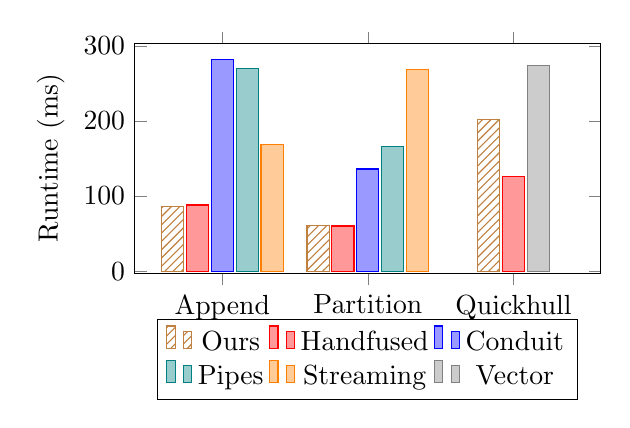
\begin{tikzpicture}
\usetikzlibrary{patterns}

% Bar chart for benchmarks:
% This is a complicated bar chart because there are six series (conduit, pipes, vector..), but they are not all defined at all points (append, partition, quickhull).
% We need to split it into three different pictures, overlaid on top of each other.
% The first picture just defines the legend, the axis labels, etc.
\begin{axis}[
  symbolic x coords={Append, Partition, Quickhull, end},
  xtick=data, ylabel=Runtime (ms),
  % All pictures need to specify same upper and lower bounds so they line up together
  ymin=0, ymax=300,
  xmin=Append, xmax=Quickhull,
        enlargelimits=0.01,
  enlarge x limits=0.30,
        ybar=1pt,
        bar width=8pt,
  width=7.5cm, height=4.5cm,
  legend style={at={(0.5,-0.2)},anchor=north, legend columns=3},
]
% The colours need to be specified manually, to force the legend entries to show up..
% The colours also need to match the colours specified for each series data.
\addlegendimage{brown,pattern=north east lines,pattern color=brown}
\addlegendimage{red,fill=red!40!white}
\addlegendimage{blue,fill=blue!40!white}
\addlegendimage{teal,fill=teal!40!white}
\addlegendimage{orange,fill=orange!40!white}
\addlegendimage{gray,fill=gray!40!white}
\legend{Ours, Handfused, Conduit, Pipes, Streaming, Vector}
\end{axis}

% This picture shows the values for Append and Partition, since they have the same series defined
\begin{axis}[
  symbolic x coords={Append, Partition, Quickhull, end},
  ticks=none,
  ymin=0, ymax=300,
  xmin=Append, xmax=Quickhull,
  enlargelimits=0.01,
  enlarge x limits=0.30,
  ybar=1pt,
  bar width=8pt,
  width=7.5cm, height=4.5cm,
]
% Ours
\addplot[brown,pattern=north east lines,pattern color=brown] coordinates {(Append,  86) (Partition,  61)   };
% Handfused
\addplot[red,fill=red!40!white] coordinates {(Append,  88) (Partition,  60)   };
% Conduit
\addplot[blue,fill=blue!40!white] coordinates {(Append, 282) (Partition, 136)   };
% Pipes
\addplot[teal,fill=teal!40!white] coordinates {(Append, 270) (Partition, 166)  };
% Streaming
\addplot[orange,fill=orange!40!white] coordinates {(Append, 168) (Partition, 268)  };
\end{axis}

% This picture shows the Quickhull results
\begin{axis}[
  symbolic x coords={Append, Partition, Quickhull, end},
  ticks=none,
  ymin=0, ymax=300,
  xmin=Append, xmax=Quickhull,
  enlargelimits=0.01,
  enlarge x limits=0.30,
  ybar=1pt,
  bar width=8pt,
  width=7.5cm, height=4.5cm,
]
% Ours
\addplot[brown,pattern=north east lines,pattern color=brown] coordinates {  (Quickhull, 202)  };
% Handfused
\addplot[red,fill=red!40!white] coordinates {  (Quickhull, 126)  };
% Vector
\addplot[gray,fill=gray!40!white] coordinates {(Quickhull, 274)  };
\end{axis}

% Runtimes for Quickhull 40MB:
% Conduit 2-pass:     300ms
% Conduit 1-pass:     264ms
% Hand:                 3ms
% Folderol:             6ms
% Vector recompute:     8ms
% Vector store:        11ms

\end{tikzpicture}
\caption{Runtime for benchmarks; lower is faster.}
\label{fig:bench:all}
\end{figure}




% %!TEX root = ../Main.tex

% -----------------------------------------------------------------------------
\section{Results}
\label{s:Benchmarks}

We have implemented this system using Template Haskell for code generation in a library called @folderol@\footnote{\url{https://github.com/amosr/folderol}}.
To better compare against existing fusion systems, we have chosen to use the finite stream extension mentioned in~\S\ref{s:Finite} for our benchmarks.
We present three benchmarks: one array benchmark, and two file-based benchmarks.

\begin{figure}
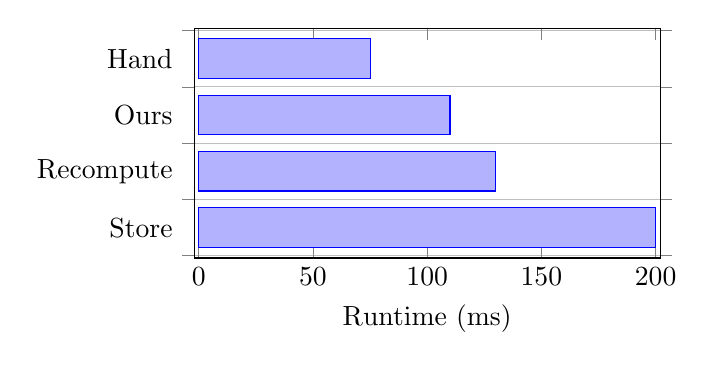
\begin{tikzpicture}
\begin{axis}[
  symbolic y coords={Store, Recompute, Ours, Hand, end},
	xlabel=Runtime (ms),
  xmin=0, xmax=200,
	enlargelimits=0.01,
	xbar interval=0.7,
  width=7.5cm, height=4.5cm,
	legend pos=north west,
]
\addplot coordinates {(200,Store) (130,Recompute) (110,Ours) (75,Hand) (0,end) };
\end{axis}
\end{tikzpicture}
\caption{Runtime for Quickhull; lower is faster.}
\label{fig:bench:quickhull}
\end{figure}

\subsection{Quickhull}
Quickhull is a divide-and-conquer spatial algorithm to find the smallest convex hull containing all points.
At its core is an operation called `filterMax', which takes a line and an array of points, and computes the maximum distance from the line, as well as all points that are above the line.
In our system this can be fused into a single loop, while shortcut-fusion systems do not support horizontal fusion.

We compare hand-fused against ours, as well as two @Data.Vector@ versions, which uses shortcut fusion.
The shortcut fusion system cannot fuse both operations into a single loop, and both operations require the distances between the line and each point.
This means a choice must be made: either compute the distances upfront and share them, or recompute the distances in each operation.
For our benchmarks we implemented both, and recomputing was significantly faster.
However, it is worth noting that we only benchmarked with two-dimensional points: at higher dimensions, the cost of recomputing distances may outweigh the cost of array allocation.

\autoref{fig:bench:quickhull} shows the runtimes for Quickhull over roughly 80MB of data, or five million points.
The hand-fused version is the fastest, while our version is slower, but still faster than the two vector versions.
The fact that our version is slower than the hand-fused version is surprising, as the generated GHC core is almost identical: the only difference is an extra continuation bound inside the loop, which acts as a sort of indirect jump in the recursive case.
It is possible that recent work on optimising continuations in GHC~\cite{downen2016sequent} will solve this.

\begin{figure}
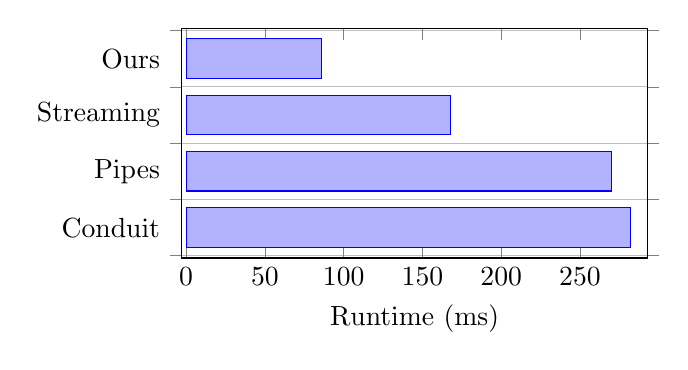
\begin{tikzpicture}
\begin{axis}[
  symbolic y coords={Conduit, Pipes, Streaming, Ours, end},
	xlabel=Runtime (ms),
  xmin=0, xmax=290,
	enlargelimits=0.01,
	xbar interval=0.7,
  width=7.5cm, height=4.5cm,
	legend pos=north west,
]
\addplot coordinates {(282,Conduit) (270,Pipes) (168,Streaming) (86,Ours) (0,end) };
\end{axis}
\end{tikzpicture}
\caption{Runtime for append2; lower is faster.}
\label{fig:bench:append}
\end{figure}

\subsection{Append files}
The first file-based benchmark consists of appending two files, while counting the number of lines.
We have benchmarked against three Haskell streaming libraries: Conduit, Pipes, and Streaming.
\autoref{fig:bench:append} shows the runtimes for appending 1.8MB of data.
The absolute performance here is poor because all are using line-buffered IO; in practice one would use chunked IO, but the overhead per chunk would remain.


\begin{figure}
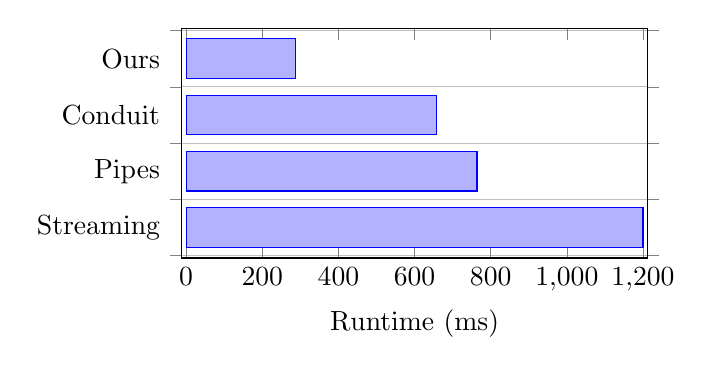
\begin{tikzpicture}
\begin{axis}[
  symbolic y coords={Streaming, Pipes, Conduit, Ours, end},
	xlabel=Runtime (ms),
  xmin=0, xmax=1200,
	enlargelimits=0.01,
	xbar interval=0.7,
  width=7.5cm, height=4.5cm,
	legend pos=north west,
]
\addplot coordinates {(1200,Streaming) (764,Pipes) (658,Conduit) (288,Ours) (0,end) };
\end{axis}
\end{tikzpicture}
\caption{Runtime for partition; lower is faster.}
\label{fig:bench:part}
\end{figure}

\subsection{Partition file}
The second file-based benchmark takes a single input file and partitions it into two files: one with even-length lines, and one with odd-length lines.
The number of lines in each output file is also counted.
The three streaming libraries are pull-based, and so do not support multiple outputs; the program must be written in a convoluted way or at least partially hand-fused.
Even with hand-fusion, the Pipes and Conduit programs are slower than ours, as well as losing any abstraction benefits from using a streaming library.
\autoref{fig:bench:part} shows the runtimes for partitioning a file into two.

%!TEX root = ../Main.tex

\section{Proofs}
\label{s:Proofs}

Our fusion system is formalised in Coq, where we have proved soundness of \ti{fusePair}: if the fused program evaluates to a particular output, then the two original programs also evaluate to that output.
It is interesting to note that the converse is not necessarily true: just because two programs can evaluate to a particular output does not mean the fused program will evaluate to that.
This is because evaluation of a process network is non-deterministic, and fusion commits to a particular evaluation order.

The problem with commiting to an evaluation order is most easily explained with a process network containing two infinitely pushing processes.
Process @A@ is repeatedly pushing to a stream called @X@, while process @B@ repeatedly pushes to @Y@.
When evaluating this pair as a process network, there are an infinite number of possible interleavings: all @X@s, all @Y@s, pairs of @X@s followed by @Y@s and so on.

When fusion is performed on this process pair, an arbitrary but \emph{particular} order will be chosen.
Thus, the chosen order will be one of the valid ones, but not all valid orders will be the chosen one.

We know of no realistic examples where combinators have multiple evaluation orders, so we believe this is not an issue in practice.

The system described here has some differences to our Coq formalisation.
First, the Coq formalisation has a separate @update@ instruction which modifies a variable in the local heap, rather than allowing heap updates in the output \Next~label of any instruction.
This causes the fusion definition to be slightly more complicated, as two output instructions must be emitted when performing a push or pull followed by an update.
This is a fairly minor difference, and we have made this change in the paper version for ease of exposition.
Ideally, a future version of the formalisation would have this change.
Secondly, our formalisation does not implement the concurrent evaluation semantics for processes, only sequential evaluation for a single process.
Instead we sequentially evaluate both processes separately with the same input values and outputs.
Finally, we have not implemented \ti{fuseNetwork} for fusing multiple processes at a time, only \ti{fusePair} for fusing pairs of processes.

Despite these differences, we believe the current formalisation gives sufficient confidence in correctness.


%!TEX root = ../Main.tex
\section{Related}
\label{s:Related}

The most closely related transforms are induction variable elimination\cite{shivers1988control} and global value numbering\cite{rosen1988global}.
Induction variable elimination finds and removes accumulators that are linear functions of the iteration number.
This does not deal with non-linear functions such as sum, or mutually recursive accumulators.

Global value numbering works on an SSA form and is much more general than induction variable elimination.
Early versions such as Rosen et al\cite{rosen1988global} only worked on extended basic blocks with backedges removed.
Alpern et al\cite{alpern1988detecting} introduced cases for specific loop backedges, where a fixpoint is performed to find the congruence sets of loops.
More recently, Gulwani and Necula\cite{gulwani2004polynomial} improved upon this, supporting removal of more expressions, and imposing a polynomial time bound.
Global value numbering for loops can perform all optimisations here.

Even better is Nie and Cheng's approach\cite{nie2007efficient}, which does not seem to be more complete or lower complexity than Gulwani and Necula, just lower constant factors.

Common subexpression elimination is very closely related, but most imperative compilers only perform common subexpression elimination on straight-line computations with no control flow\cite{debray1992compiler}, or on loop invariant expressions\cite{bodik1998complete}.
Common subexpression elimination for functional languages would be able remove lone expressions, but does not deal with mutually recursive folds.

Temporal common subexpression elimination in Single Assignment C
allows reuse of expressions computed in the previous iteration\cite{imlig2001loop}.
This is a more general case of the elimination opportunities that arise from loop unrolling.

For example, the program below loops over an array @A@, and stores the product @a@ of some computation on the current element (@f(A[i])@), while performing the same computation over the next element (@f(A[i+1])@) and summing it in @b@.
On successive iterations, the @bx = f(A[i+1])@ computed from last iteration could be reused as the new @ax = f(A[i])@.
\begin{code}
int[] A;
int a = 1;
int b = 0;
while(int i = 0; i != size - 1; i++)  {
  int ax = f(A[i]);
  int bx = f(A[i+1]);
  a += ax;
  b *= bx;
}
\end{code}

I cannot think of a better example than this right now.

Continuous queries are a similar domain, where a single query keeps running and producing results, as data is received.
In \cite{munagala2007optimization} there are multiple queries based off the same incoming stream.
Each queries is filtered by a conjunction of predicates, where each single predicate may be used by multiple queries.
If these predicates are expensive to compute, it is certainly not ideal to compute these for each query.

Multi-query data analysis\cite{andrade2003efficient} describes a similar problem, where they have multiple queries over the same data that run periodically.
By grouping the multiple queries together, more optimisations can be performed than when treating the queries separately.
This is a lot closer, and performs CSE on expressions like @x = sum(y)@, where @sum@ is a built-in aggregate function.
However, this is only for a small set of built-in aggregates, and does not deal with mutually recursive definitions.


The polyhedral model\cite{benabderrahmane2010polyhedral} analyses data dependencies in loops.
For a given iteration, the polyhedral model computes the iterations which must be executed before the given iteration.
By knowing the dependent iterations, one can restructure the loop so that the iterations are executed in a different order, while still performing any dependencies in order.
For example, a loop iterating over @i@, with loop body @A[i] = A[i-10]@ depends on the tenth previous iteration.
This loop could be executed in an order like @0, 1, 2,...@, but it could also stride by ten: @0, 10, 20..., 1, 11, 21,...@.
This allows fusion of any two loops if the intersection of the two loops' iteration spaces is not empty.
In our case the iteration order is fixed, as the program cannot control the order in which stream elements are received.
The polyhedral model may still be applicable to streaming computations where one could introduce certain-sized buffers, then process the buffer in parallel.
In this case the polyhedral model may expose more opportunities for duplicate elimination, but does not itself remove duplicates.


% %!TEX root = ../Main.tex
\section{Conclusions and future work}
\label{s:FutureWork}

We now discuss some of the shortcomings of the system, and extensions and future work to ameliorate this.

\subsection{Finite streams}
\label{s:Finite}

The processes we have seen so far deal with infinite streams, but in practice most streams are finite.
Certain combinators such as @fold@ and @append@ only make sense on finite streams, and others like @take@ produce inherently finite output.
We have focussed on the infinite stream version because it is somewhat simpler to explain and prove, but the extensions required to support finite streams do not require substantial conceptual changes.

We now describe the extensions required to support finite streams.
We add a new @closed@ constructor to the \InputState~ to encode the end of the stream.
Once an input stream is in the closed state, it can never change to another state: it remains closed thereafter.

We modify the @pull@ instruction so that it has two output labels (like @case@).
The first label, the read branch, is executed as before when the pull succeeds and a value is read from the stream.
The second label, the close branch, is executed when the stream is closed, and no more values will ever be available.
After a pull takes the close branch, any subsequent pulls from that stream will also take the close branch.

We add two new instructions for closing output streams and disconnecting from input streams.
Closing an output stream $(@close@~\Chan~\Goto)$ is similar to pushing an end-of-file marker to all readers.
As with @push@, the evaluation semantics of @close@ can only proceed if all readers are in a position to accept the end-of-file, but instead of setting the new \InputState~ to @pending@ with a value, the \InputState~ is set to @closed@.
After a stream has been closed, no further values can be pushed.

Disconnecting from input streams $(@disconnect@~\Chan~\Goto)$ signals that a process is no longer interested in the values of a stream.
This can be used when a process requires the first values of a stream, but does not require the whole stream.
If a process read the first values of a stream and then stopped pulling, its \InputState~ buffer would fill up and never be cleared, so no other process would be able to continue pulling from that stream.
Disconnecting the stream allows other processes to use the stream without the disconnected process getting in the way of computation.
The evaluation semantics for @disconnect@ remove the channel from the inputs of the process.
After removing the channel from the inputs, when a writing process tries to inject values, this process will just be ignored rather than inserting into the \InputState~ buffer and potentially causing writing to block.
After a process disconnects from an input channel, it can no longer pull from that channel.

We also add an instruction for terminating the process (@done@).
After all input streams have been read to completion or disconnected and output streams closed, the process may execute @done@ to signal that processing is complete.

The fusion definition must be extended to deal with these new instructions.
The static input state has a @closed@ constructor added and disconnection is encoded by removal from the input state, and the \ti{tryStep} changes more or less follow the evaluation changes.
Shared and connected pulls now deal with two more possibilities in the input state: the input may be closed in which case the close branch of the pull is taken; or the other process may have disconnected in which case the pull is executed as in the non-shared non-connected case.
Connected pushes must also deal with when the other process has disconnected in which case the push is executed as if it were non-connected.
For @in1@ and @out1@ channels, the new @close@ and @disconnect@ instructions are used as normal with no coordination required.
For connected @close@, as with @push@, the receiving process must have @none@ and the next step performs the @close@ and sets the input state to @closed@.
For shared @disconnect@, the @disconnect@ is only performed after both processes have disconnected; otherwise the entry is just removed from the input state.
For connected @disconnect@, the @disconnect@ is not performed and the entry is removed from the input state.

Finally, \ti{tryStepPair} is modified so that @done@ is performed when both machines are @done@.

These modifications allow our system to fuse finite streams as well as infinite.
We have implemented an initial prototype that supports finite streams, but future work is required to prove them correct.

\subsection{Fully abstract case interpretation}
\label{s:FullyAbstractCase}

The fusion algorithm treats all @case@ conditions as fully abstract, by exploring all possible combinations for both processes.
This can cause an issue with coordination and buffering, as the processes may dynamically require only a bounded buffer, the fusion algorithm statically tries every combination and wrongly asserts that unbounded buffering is required.

For example, suppose two processes have the same case condition @x > 0@.
The fusion algorithm will try all possibilities including contradictory ones, such as where the first process has @x > 0 = true@ and the second has @x > 0 = false@.
If any of these possibilities require an unbounded buffer, the fusion algorithm fails.
This means that the following program which pairs all positive elements with themselves, while unlikely to be written by a human, is not able to be fused.
\begin{code}
zipgts as =
  let as1 = filter (>0) as
      as2 = filter (>0) as
      aas = zip as1 as2
  in  aas
\end{code}

In general, if the example above used two different predicates for each filter, the fusion system would be right to outlaw it as requiring unbounded buffers.
If the same program is rewritten to use only a single filter and use its result twice, the program is able to be fused.

A possible extension is to somehow cull these contradictory states so that if it is statically known that a state is unreachable, it does not matter if it requires unbounded buffers.
It may be possible to achieve this with relatively little change to the fusion algorithm itself, by having it emit some kind of failure instruction rather than failing to produce a process.
A separate postprocessing step could then perform analyses and remove statically unreachable process states.
After postprocessing, if any failure instructions are reachable, the fusion process would fail as before.

\subsection{Non-determinism and fusion order}
\label{s:FusionOrder}

The main fusion algorithm here works on pairs of processes.
When there are more than two processes, there are multiple orders in which the pairs of processes can be fused.
The order in which pairs of processes are fused does not affect the output values, but it does affect the access pattern: the order in which outputs are produced and inputs read.
Importantly, the access pattern also affects whether fusion succeeds or fails to produce a process.
In other words, while evaluating multiple processes is non-deterministic, the act of fusing two processes \emph{commits} to a particular deterministic interleaving of the two processes.
The simplest example of this has two input streams, a function applied to both, then zipped together. 

\begin{code}
zipMap as bs =
  let as' = map (+1) as
      bs' = map (+1) bs
      abs = zip as' bs'
  in  abs
\end{code}

There are three combinators here, so after converting each combinator to its process there are three orders we can fuse.
The two main options are to fuse the two maps together and then add the zip, or to fuse the zip with one of the maps, then add the other map.
If we start by fusing the zip with one of its maps, the zip ensures that its inputs are produced in lock-step pairs, and then adding the other map will succeed.
However if we try to fuse the two maps together, there are many possible interleavings: the fused program could read all of @as'@ first; it could read all of @bs'@ first; it read the two in lock-step pairs; or any combination of these.
When the zip is added, fusion will fail if the wrong interleaving was chosen.

% The example above can be solved by fusing connected processes first, but it is possible to construct a connected process that still relies on the order of fusion.
% 
% \begin{code}
% zipApps as bs cs =
%   let as' = as ++ bs
%       bs' = as ++ cs
%       abs = zip as' bs'
%   in  abs
% \end{code}

Our current solution to this is to try all permutations of fusing processes and use the first one that succeeds.
A more principled solution may be to allow non-determinism in a single process by adding a non-deterministic choice instruction.
Then when fusing two processes together, if both processes are pulling from unrelated streams, the result would be a non-deterministic choice between pulling from the first process and executing the first, or pulling from the second process and executing the second.
In this way we could defer committing to a particular evaluation order until the required order is known.
This may produce larger intermediate programs, but the same deterministic program could be extracted at the end.



\bibliography{Main}

%%% "Extended paper"
% \appendix
% %!TEX root = ../Main.tex
\eject
\appendix

\section{Finite streams}
\label{s:FiniteDetails}

This appendix briefly describes the finite streams extension, showing the changes to instructions and the fusion algorithm.
The finite evaluation rules are not shown, as the changes follow the same structure as the changes to the fusion algorithm.

\begin{figure}
\begin{tabbing}
MMMMMM \TABDEF @MMMMM@  \TABSKIP $\Chan$ \TABSKIP $\Chan$ \TABSKIP $\Next$ \TABSKIP \kill
\Instr
    \> ::=\> @push@  \> \Chan  \> \Exp  \> \Next \\
    \TABALT  @drop@  \> \Chan  \>       \> \Next \\
    \TABALT  @case@  \> \Exp   \> \Next \> \Next \\
    \TABALT  @jump@  \>        \>       \> \Next \\
    \\
    \TABALT  @pull@  \> \Chan  \> \Var  \> \Next \> \Next \\
    \TABALT  @close@ \> \Chan  \>       \> \Next \\
    \TABALT  @exit@ 
\\
\\
$\InputState_F$ \> ::=  \> ~~~ $@none@_F ~|~ @pending@_F ~|~ @have@_F ~|~ @closed@_F$
\end{tabbing}
\caption{Finite instructions}
\label{fig:Finite:Instr}
\end{figure}

Figure~\ref{fig:Finite:Instr} shows the grammar for instructions and the static input state. The first group of instructions containing @push@, @drop@, @case@ and @jump@ are unchanged.

The @pull@ instruction is modified to have two output labels, similar to @case@. The first, the success branch, is used when the input stream is still open and pulling succeeds, in which case the variable is set to the pulled value as before. The second output label, the closed branch, is used when the input stream has been closed, and the variable is not written to. This new @pull@ is analogous to a @pull@ followed by a @case@ in the infinite stream version.

The @close@ instruction is used by a pushing process to close or end an output stream. Any subsequent pulls from this channel in other processes will take the closed branch. After an output channel is closed, it cannot be pushed to and remains closed forever.

Finally, the @exit@ instruction is used once a process is finished with all its streams, and has nothing left to do. All output streams must be closed before the process finishes. This instruction has no output labels, as there is nothing further to execute.

Also in Figure~\ref{fig:Finite:Instr}, the static input state used for fusion ($\InputState_F$) must now track closed streams. The new constructor $@closed@_F$ denotes that the stream is closed, while the rest is unchanged.

For the fusion algorithm, the top-level function $\ti{fusePair}$ remains unchanged. The functions $\ti{outlabels}$ and $\ti{swaplabels}$ are not shown as they are easily modified by adding cases for the new instructions.

Figure~\ref{fig:Finite:tryStepPair} shows the modified $\ti{tryStepPair}$ function. This function uses the same heuristics to decide which process to execute when both can progress, but now that the processes can finish with @exit@, we must take care to only finish the fused process once \emph{both} source processes are finished. The (DeferExit1) and (DeferExit2) clauses achieve this by forcing the other process to run if one is an @exit@. Once both processes are finished, both new clauses will fail while (DeferPull1) succeeds, using the @exit@ from the first process. Another way to think of this is that if either process has work to do, the fused process still has work to do.

\begin{figure}
\begin{tabbing}
M \= M \= M \= MMMMMMMMMMMMMMMMMMM \= \kill
$\ti{tryStepPair} ~:~ \ChanTypeMap$ \\
\> \> $\to \Label_1 \to \Instr$ ~~~
            $\to \Label_1 \to \Instr$ \\
\> \> $\to \Maybe~\Instr$ \\
$\ti{tryStepPair} ~\cs~l_p~i_p~l_q~i_q$ \\

\> $~|~i_p'~\in~\ti{tryStep}~\cs~l_p~i_p~l_q ~\wedge~ i_q'~\in~\ti{tryStep}~\cs~l_q~i_q~l_p$ \\
\> ~~ $\wedge~@exit@~\not\in~i_p'$ 
   ~~~~~ $\to~i_p'$ 
\> \> \> \note{DeferExit1} 
\\[0.5ex]

\> $~|~i_p'~\in~\ti{tryStep}~\cs~l_p~i_p~l_q ~\wedge~i_q'~\in~\ti{tryStep}~\cs~l_q~i_q~l_p$ \\
\> ~~ $\wedge~@exit@~\not\in~i_q'$ 
   ~~~~~ $\to~\ti{swaplabels}~i_q'$ 
\> \> \> \note{DeferExit2} 
\\[0.5ex]


\> $~|~i_p'~\in~\ti{tryStep}~\cs~l_p~i_p~l_q ~\wedge~@jump@~(l,u)~\in~i_p'$ \\
\> $\to~i_p'$
\> \> \> \note{PreferJump1} 
\\[0.5ex]

\> $~|~i_q'~\in~\ti{tryStep}~\cs~l_q~i_q~l_p ~\wedge~@jump@~(l,u)~\in~i_q'$ \\
\> $\to~\ti{swaplabels}~i_q'$ 
\> \> \> \note{PreferJump2}
\\[0.5ex]

\> $~|~i_p'~\in~\ti{tryStep}~\cs~l_p~i_p~l_q ~\wedge~ i_q'~\in~\ti{tryStep}~\cs~l_q~i_q~l_p$ \\
\> ~~ $\wedge~@pull@~c~x~(l,u)~\not\in~i_p'$ 
   ~~~~~ $\to~i_p'$ 
\> \> \> \note{DeferPull1} 
\\[0.5ex]

\> $~|~i_p'~\in~\ti{tryStep}~\cs~l_p~i_p~l_q ~\wedge~i_q'~\in~\ti{tryStep}~\cs~l_q~i_q~l_p$ \\
\> ~~ $\wedge~@pull@~c~x~(l,u)~\not\in~i_q'$ 
   ~~~~~ $\to~\ti{swaplabels}~i_q'$ 
\> \> \> \note{DeferPull2} 
\\[0.5ex]

\> $~|~i_p'~\in~\ti{tryStep}~\cs~l_p~i_p~l_q$ ~~~~~ $\to~i_p'$ 
\> \> \> \note{Run1} 
\\[0.5ex]

\> $~|~i_q'~\in~\ti{tryStep}~\cs~l_q~i_q~l_p$ ~~~~~ $\to~\ti{swaplabels}~i_q'$
\> \> \> \note{Run2} \\


\end{tabbing}
\caption{Fusion step coordination for a pair of processes.}
\label{fig:Finite:tryStepPair}
\end{figure}

Figure~\ref{fig:Finite:tryStep} shows the modified $\ti{tryStep}$ function.
The clauses for the unchanged instructions @push@, @drop@, @case@ and @jump@ remain unchanged; these are reordered to the top of the function.

The @pull@ clauses use $l'_o$ for the open output label, and $l'_c$ for the closed label.
Clause (LocalPull) now uses two output labels, and leaves the other process as-is.

Clause (SharedPull) applies when the channel state is @pending@, meaning there is already a value available. This means that the channel is not yet closed, and the success branch can be taken.

Clause (SharedPullInject) applies when both processes need to pull from a shared input. As before, we execute a real @pull@, this time with two branches. In the success branch, the input states are set to @pending@ as before. In the closed branch, the input states are set to @closed@ so the next and subsequent pulls take the closed branch.

Clause (SharedPullClosed) applies when the channel state is @closed@, which means either the other process has pulled and discovered that the channel is closed, or in case of connected input, the other process has closed the channel. Either way we simply jump, taking the closed branch of the @pull@.

Clause (LocalClose) applies when closing a local output.

Clause (SharedClose) applies when closing a connected output. As with (SharedPush), the other input state for the other process must be empty and ready to pull from the channel. The input state for the other process is then set to @closed@, forcing its next pull to take the closed branch.

Finally, clause (LocalExit) allows the process to finish. However, recall that the $\ti{tryStepPair}$ function has been modified to only @exit@ when both processes are ready to finish.

\begin{figure*}
\begin{tabbing}
M \= M \= MMMMMMMMMMMMMMMMMMMMMM \= MMMMMMMMMMMMMMMMMMMMMMMMMMMMMM \= \kill
$\ti{tryStep} ~:~ \ChanTypeMap \to \Label_1 \to \Instr \to \Label_1 \to \Maybe~\Instr$ \\
$\ti{tryStep} ~\cs~(l_p,s_p)~i_p~(l_q,s_q)~=~@match@~i_p~@with@$ \\

\> $@jump@~(l',u')$ 
\> \> $\to~@jump@~
      \nextStep
        {l'}{s_p}
        {l_q}{s_q}
        {u'}
      $ 
\> \note{LocalJump}
\\[1ex]

\> $@case@~e~(l'_t,u'_t)~(l'_f,u'_f)$
\> \> $\to~@case@~e~
      \nextStep
        {l'_t}{s_p}
        {l_q}{s_q}
        {u'_t}
      ~
      \nextStep
        {l'_f}{s_p}
        {l_q}{s_q}
        {u'_f}
      $ 
\> \note{LocalCase}
\\[1ex]

\> $@push@~c~e~(l',u')$ \\
\> \> $~|~\cs[c]=@out1@$ 
\> $\to~@push@~c~e~
      \nextStep
        {l'}
          {s_p}
        {l_q}
          {s_q}
        {u'}
      $ 
\> \note{LocalPush}\\

\> \> $~|~\cs[c]=@in1out1@ ~\wedge~ s_q[c]=@none@_F$ 
\> $\to~@push@~c~e~
      \nextStep
        {l'}
          {s_p}
        {l_q}
          {\HeapUpdateOne{c}{@pending@_F}{s_q}}
        {\HeapUpdateOne{@chan@~c}{e}{u'}}
      $
\> \note{SharedPush}
\\[1ex]

\> $@drop@~c~(l',u')$ \\
\> \> $~|~\cs[c]=@in1@$
\> \hspace{2em} $\to~@drop@~c~
      \nextStep
        {l'}
          {s_p}
        {l_q}
          {s_q}
        {u'}
      $
\> \note{LocalDrop} \\

\> \> $~|~\cs[c]=@in1out1@$
\> \hspace{2em} $\to~@jump@~
      \nextStep
        {l'}
          {\HeapUpdateOne{c}{@none@_F}{s_p}}
        {l_q}
          {s_q}
        {u'}
      $
\> \note{ConnectedDrop}\\

\> \> $~|~\cs[c]=@in2@ ~\wedge~ (s_q[c]=@have@_F \vee s_q[c]=@pending@_F)$ 
\> \hspace{2em} $\to~@jump@~
      \nextStep
        {l'}
          {\HeapUpdateOne{c}{@none@_F}{s_p}}
        {l_q}
          {s_q}
        {u'}
      $
\> \note{SharedDropOne}\\



\> \> $~|~\cs[c]=@in2@ ~\wedge~ s_q[c]=@none@_F$
\> \hspace{2em} $\to~@drop@~c~
      \nextStep
        {l'}
          {\HeapUpdateOne{c}{@none@_F}{s_p}}
        {l_q}
          {s_q}
        {u'}
      $
\> \note{SharedDropBoth}
\\[1ex]

\\



\> $@pull@~c~x~(l'_o,u'_o)~(l'_c,u'_c)$ \\
\> \> $~|~\cs[c]=@in1@$ 
\> $\to~@pull@~c~x~
      \nextStep
        {l'_o}{s_p}
        {l_q}{s_q}
        {u'_o}
      ~
      \nextStep
        {l'_c}{s_p}
        {l_q}{s_q}
        {u'_c}
    $ 
\> \note{LocalPull}
\\[1ex]

\> \> $~|~(\cs[c]=@in2@ \vee \cs[c]=@in1out1@) ~\wedge~ s_p[c]=@pending@_F$ \\
\> \> $\to~@jump@~
      \nextStep
        {l'_o}
          {\HeapUpdateOne{c}{@have@_F}{s_p}}
        {l_q}
          {s_q}
        {\HeapUpdateOne{x}{@chan@~c}{u'_o}}
        $ 
\> \> \note{SharedPull} 
\\[1ex]

\> \> $~|~\cs[c]=@in2@ ~\wedge~ s_p[c]=@none@_F ~\wedge~ s_q[c]=@none@_F$ \\
\> \> $\to~@pull@~c~(@chan@~c)~
      \nextStep
        {l_p}
          {\HeapUpdateOne{c}{@pending@_F}{s_p}}
        {l_q}
          {\HeapUpdateOne{c}{@pending@_F}{s_q}}
        {[]}$
      \\
\> \> @                @
      $\nextStep
        {l_p}
          {\HeapUpdateOne{c}{@closed@_F}{s_p}}
        {l_q}
          {\HeapUpdateOne{c}{@closed@_F}{s_q}}
        {[]}
  $
\> \> \note{SharedPullInject}
\\[1ex]

\> \> $~|~(\cs[c]=@in2@ \vee \cs[c]=@in1out1@) ~\wedge~ s_p[c]=@closed@_F$ \\
\> \> $\to~@jump@~
      \nextStep
        {l'_c}{s_p}
        {l_q}{s_q}
        {u'_c}
  $
\> \> \note{SharedPullClosed}
\\[1ex]

\> $@close@~c~(l',u')$ \\
\> \> $~|~\cs[c]=@out1@$ 
\> $\to~@close@~c~
      \nextStep
        {l'}{s_p}
        {l_q}{s_q}
        {u'}
    $ 
\> \note{LocalClose}
\\

\> \> $~|~\cs[c]=@in1out1@ ~\wedge~ s_q[c]=@none@_F$ 
\> $\to~@close@~c~
      \nextStep
        {l'}{s_p}
        {l_q}{\HeapUpdateOne{c}{@closed@_F}{s_q}}
        {u'}
    $ 
\> \note{SharedClose}
\\[1ex]

\> $@exit@$
\> 
\> $\to~@exit@$
\> \note{LocalExit}
\\


\end{tabbing}

\caption{Fusion step for a single process of the pair.} 

\label{fig:Finite:tryStep}
\end{figure*}


% %!TEX root = ../Appendix.tex

\clearpage{}
\section{Result Size}
\label{s:ResultSize}

As with any fusion system, we must be careful that the size of the result code does not become too large when more and more processes are fused together. 

\subsection{Fusing Pipelines of Processes}
The following figure shows the maximum number of output states in the result when a particular number of processes are fused together in a pipelined-manner.

\smallskip
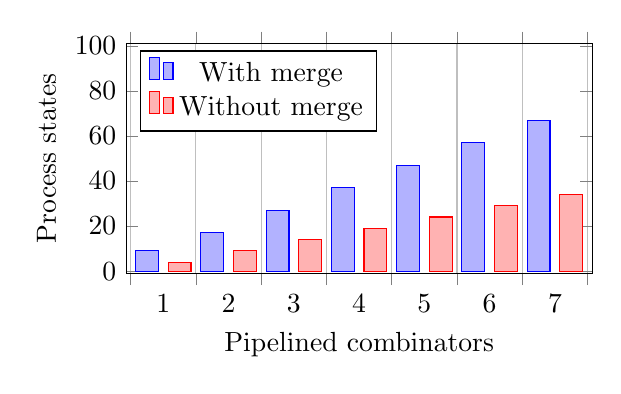
\begin{tikzpicture}
\begin{axis}[
% Hide the label on the second graph
        ylabel=Process states,
        xlabel=Pipelined combinators,
  ymin=0, ymax=100,
        enlargelimits=0.01,
        ybar interval=0.7,
  width=7.5cm, height=4.5cm,
        legend pos=north west,
]
\addplot coordinates {(1,9) (2,17) (3,27) (4,37) (5,47) (6,57) (7,67)   (8,1) };
\addplot coordinates {(1,4) (2,9) (3,14) (4,19) (5,24) (6,29) (7,34)    (8,1) };
\legend{With merge, Without merge};
\end{axis}
\end{tikzpicture}


To produce the above graph we programmatically generated dataflow networks for \emph{all possible} pipelined combinations of the @map@, @filter@, @scan@, @group@ and @merge@ combinators, and tried all possible fusion orders consiting of adjacent pairs of processes. The @merge@ combinator itself has two inputs, so only works at the very start of the pipeline --- we present result for pipelines with and without a @merge@ at the start. 

\subsection{Fusing Parallel Processes}
The following figure shows the number of states in the result when the various combinations of combinators are fused in parallel, for example, we might have a @map@ and a @filter@ processing the same input stream. In both cases the number of states in the result process grows linearly with the number of processes. In all combinations, with up to 7 processes there are less than 100 states in the result process.

\smallskip
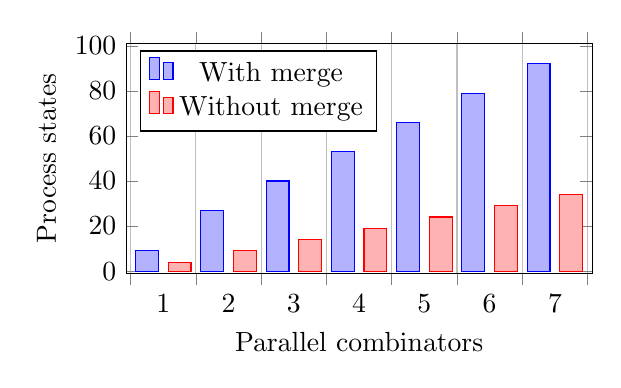
\begin{tikzpicture}
\begin{axis}[
        ylabel=Process states,
        xlabel=Parallel combinators,
  ymin=0, ymax=100,
        enlargelimits=0.01,
        ybar interval=0.7,
  width=7.5cm, height=4.5cm,
        legend pos=north west,
]
\addplot coordinates {(1,9) (2,27) (3,40) (4,53) (5,66) (6,79) (7,92)
  % Last bar doesn't show for some reason, so need to add a dummy value for the next one
    (8,1) };

\addplot coordinates {(1,4) (2,9) (3,14) (4,19) (5,24) (6,29) (7,34)    (8,1) };

\legend{With merge, Without merge};
\end{axis}
\end{tikzpicture}

The size of the result process is roughly what one would get when inlining the definitions of each of the original source processes. This is common with other systems based on inlining and/or template meta-programming, and is not prohibitive.


\eject{}
% -----------------------------------------------------------------------------
\subsection{Fusing Merges}

On the other hand, the following figure shows the results for a pathological case where the size of the output program is exponential in the number of input processes. The source dataflow networks consists of N merge processes, N+1 input streams, and a single output stream. The output of each merge process is the input of the next, forming a chain of merges. In source notation the network for N = 3 is @sOut = merge sIn1 (merge sIn2 (merge sIn3 sIn4))@.

\medskip
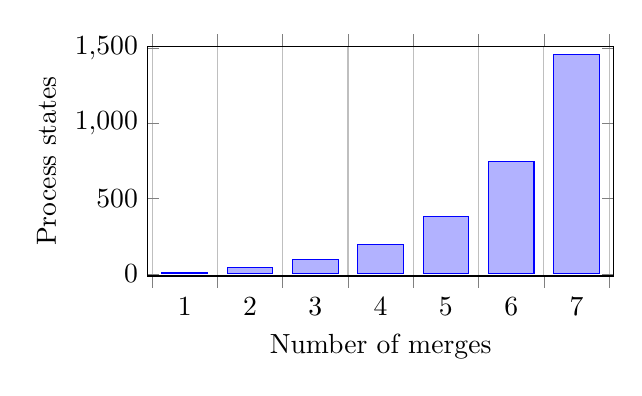
\begin{tikzpicture}
\begin{axis}[
        ylabel=Process states,
        xlabel=Number of merges,
%  ymode=log,
  ymin=0, ymax=1500,
        enlargelimits=0.01,
        ybar interval=0.7,
  width=7.5cm, height=4.5cm,
        legend pos=north west,
]
% These are the values for splitting.
% They are smaller than the 'chaining', but look much nicer on the linear graph.
\addplot coordinates {(1,9) (2,42) (3,97) (4,196) (5,383) (6,746) (7,1461)
  % (8,2880)
  (8,1)
  };

% These are the values for chaining
% \addplot coordinates {(1,4) (2,48) (3,194) (4,760) (5,2814) (6,10064) (7,1) };

\end{axis}
\end{tikzpicture}


When fusing two processes the fusion algorithm essentially compares every state in the first process with every state in the second, computing a cross product. During the fusion transform, as states in the result process are generated they are added to a finite map --- the @instrs@ field of the process definition. The use of the finite map ensures that identical states are always combined, but genuinely different states always make it into the result. 
In the worst case, fusion of two processes produces O($n*m$) different states, where $n$ and $m$ are the number of states in each. If we assume the two processes have about the same number of states then this is O($n^2$). Fusing the next process into this result yields O($n^3$), so overall the worst case number of states in the result will be O($n^k$), where $k$ is the number of processes fused. 

In the particular case of @merge@, the implementation has two occurrences of the @push@ instruction. During fusion, the states for the consuming process are inlined at each occurrence of @push@. These states are legitimately different because at each occurence of @push@ the input channels of the merge process are in different channel states, and these channel states are included in the overall process state.


% \clearpage{}
% %!TEX root = ../Appendix.tex
\clearpage{}

\section{Combinators}
\label{s:Combinators}
Here we show the definitions of some combinators. We start with simple combinators supported by most streaming systems, and progress to more interesting combinators. Some standard combinators such as @fold@, @take@ and @append@ are missing due to the infinite nature of our streams, but could be implemented with the finite stream extension. The fact that segmented versions of these combinators can be implemented is compelling evidence of this.

Many of these combinators take a ``default'' argument, which is used to initialise the heap, but the stored value is never actually read. Ideally these could be left unspecified, or the heap left uninitialised in cases where it is never read.

\subsection{Map}
The map combinator applies a function to every element of the stream. This is some more text.

\begin{alltt}
map 
 =  \(\lambda\) (f : \(\alpha \to \beta\)) (default : \(\alpha\))
      (sIn: Stream \(\alpha\)) (sOut: Stream \(\beta\)). 
    \(\nu\) (a: \(\alpha\)) (L0..L2: Label).
\end{alltt}
\begin{code}
    process
    { ins:    { sIn }
    , outs:   { sOut }
    , heap:   { a = default }
    , label:  L0
    , instrs: { L0 = pull sIn     a  L1 []
              , L1 = push sOut (f a) L2 []
              , L2 = drop sIn        L0 [] } }
\end{code}


% -----------------------------------------------------------------------------
\subsection{Filter}
Filter returns a new stream containing only the elements that satisfy some predicate.
\begin{alltt}
filter 
 =  \(\lambda\) (f : \(\alpha \to\) Bool) (default : \(\alpha\))
      (sIn: Stream \(\alpha\)) (sOut: Stream \(\alpha\)). 
    \(\nu\) (a: \(\alpha\)) (L0..L3: Label).
\end{alltt}
\begin{code}
    process
    { ins:    { sIn }
    , outs:   { sOut }
    , heap:   { a = default }
    , label:  L0
    , instrs: { L0 = pull sIn  a     L1 []
              , L1 = case   (f a)    L2 []  L3 []
              , L2 = push sOut a     L3 []
              , L3 = drop sIn        L0 [] } }
\end{code}


\vspace{12em}
% -----------------------------------------------------------------------------
\subsection{Partition}
Partition is similar to filter, but has two output streams: those that satisfy the predicate, and those that do not. Partition is an inherently push-based operation, and cannot be supported by pull streams without buffering.
\begin{alltt}
partition 
 =  \(\lambda\) (f : \(\alpha \to\) Bool) (default : \(\alpha\))
      (sIn:   Stream \(\alpha\))
      (sOut1: Stream \(\alpha\)) (sOut2: Stream \(\alpha\)). 
    \(\nu\) (a: \(\alpha\)) (L0..L4: Label).
\end{alltt}
\begin{code}
    process
    { ins:    { sIn }
    , outs:   { sOut1, sOut2 }
    , heap:   { a = default }
    , label:  L0
    , instrs: { L0 = pull sIn   a    L1 []
              , L1 = case    (f a)   L2 []  L3 []
              , L2 = push sOut1 a    L4 []
              , L3 = push sOut2 a    L4 []
              , L4 = drop sIn        L0 [] } }
\end{code}


% -----------------------------------------------------------------------------
\subsection{Zip}
Zip, or zip-with, pairwise combines two input streams.
Zipping is an inherently pull-based operation.

\begin{alltt}
zipWith 
 =  \(\lambda\) (f : \(\alpha \to \beta \to \gamma\)) (default1 : \(\alpha\)) (default2 : \(\beta\))
      (sIn1: Stream \(\alpha\)) (sIn2: Stream \(\beta\))
      (sOut: Stream \(\gamma\)). 
    \(\nu\) (a: \(\alpha\)) (b : \(\beta\)) (L0..L4: Label).
\end{alltt}
\begin{code}
    process
    { ins:    { sIn1, sIn2 }
    , outs:   { sOut }
    , heap:   { a = default1, b = default2 }
    , label:  L0
    , instrs: { L0 = pull sIn1 a       L1 []
              , L1 = pull sIn2 b       L2 []
              , L2 = push sOut (f a b) L3 []
              , L3 = drop sIn1         L4 []
              , L4 = drop sIn2         L0 [] } }
\end{code}


% -----------------------------------------------------------------------------
\subsection{Scan}
Scan is similar to a fold, but instead of returning a single value at the end, it returns an intermediate value for each element of the stream.

\begin{alltt}
scan 
 =  \(\lambda\) (k : \(\alpha \to \beta \to \beta\)) (z : \(\beta\)) (default : \(\alpha\))
      (sIn: Stream \(\alpha\)) (sOut: Stream \(\beta\)).
    \(\nu\) (a: \(\alpha\)) (s : \(\beta\)) (L0..L2: Label).
\end{alltt}
\begin{code}
    process
    { ins:    { sIn  }
    , outs:   { sOut }
    , heap:   { a = default, s = z }
    , label:  L0
    , instrs: { L0 = pull sIn  a   L1 []
              , L1 = push sOut s   L2 [ s = f a s ]
              , L2 = drop sIn      L0 [] } }
\end{code}


% -----------------------------------------------------------------------------
\subsection{Segmented Fold}
Segmented fold performs a fold over each nested stream, using a segmented representation.
Here we are representing nested streams using one stream for the lengths of each substream, and another stream containing the values.
The output stream has the same rate as the lengths stream.
It reads a count (@c@) from the lengths stream, setting the fold state to zero (@z@).
Then it reads count times from the values stream, updating the fold state.
Afterwards, it pushes the final fold state, and continues to read a new count.

\begin{alltt}
folds 
 =  \(\lambda\) (k : \(\alpha \to \beta \to \beta\)) (z : \(\beta\)) (default : \(\alpha\))
      (sLens: Stream Nat) (sVals: Stream \(\alpha\))
      (sOut:  Stream \(\beta\)).
    \(\nu\) (c : Nat) (a: \(\alpha\)) (s : \(\beta\)) (L0..L5: Label).
\end{alltt}
\begin{code}
    process
    { ins:    { sLens, sVals }
    , outs:   { sOut }
    , heap:   { c = 0, a = default, s = z }
    , label:  L0
    , instrs: { L0 = pull sLens c   L1 [ s = z ]
              , L1 = case (c > 0)   L2 []  L4 []
              , L2 = pull sVals a   L3 []
              , L3 = drop sVals     L1 [ c = c - 1
                                       , s = k s a ]
              , L4 = push sOut  s   L5 []
              , L5 = drop sLens     L0 [] } }
\end{code}


% -----------------------------------------------------------------------------
\subsection{Segmented Take}
Segmented take computes an @n@-length prefix of each nested stream.
It starts by reading a count from the lengths stream, then copies at most @n@ elements.
If there are leftovers, it pulls and discards them, then pulls the next length.

\begin{alltt}
takes 
 =  \(\lambda\) (n : Nat) (default : \(\alpha\))
      (sLens: Stream Nat) (sVals: Stream \(\alpha\))
      (oLens: Stream Nat) (oVals: Stream \(\alpha\)).
    \(\nu\) (c : Nat) (take : Nat) (ix : Nat) (a: \(\alpha\))
      (L0..L9: Label).
\end{alltt}
\begin{code}
    process
    { ins:    { sLens, sVals }
    , outs:   { oLens, oVals }
    , heap:   { c = 0, take = 0, ix = 0, a = default }
    , label:  L0
    , instrs: { L0 = pull sLens c     L1 
                          [ ix = 0, take = min count n ]
              , L1 = push oLens take  L2 []
              , L2 = case (ix < take) L3 []  L6 []
              , L3 = pull sVals a     L4 []
              , L4 = push oVals a     L5 []
              , L5 = drop sVals       L2 [ix = ix+1]
              , L6 = case (ix < c)    L7 []  L9 []
              , L7 = pull sVals a     L8 []
              , L8 = drop sVals       L6 [ix = ix+1]
              , L9 = drop sLens       L0 [] } }
\end{code}


% -----------------------------------------------------------------------------
\subsection{Segmented Append}
Segmented append takes two segmented streams as input, and appends each nested stream.
It starts by reading a length from both lengths streams into @a@ and @b@, and pushes the sum of both lengths.
It then copies over @a@ elements from the first values stream, then copies over @b@ elements from the second values stream.

\begin{alltt}
appends 
 =  \(\lambda\) (default : \(\alpha\))
      (aLens: Stream Nat) (aVals: Stream \(\alpha\))
      (bLens: Stream Nat) (bVals: Stream \(\alpha\))
      (oLens: Stream Nat) (oVals: Stream \(\alpha\)).
    \(\nu\) (a : Nat) (b : Nat) (v: \(\alpha\)) (L0..L12: Label).
\end{alltt}
\begin{code}
    process
    { ins:    { aLens, aVals, bLens, bVals }
    , outs:   { oLens, oVals }
    , heap:   { a = 0, b = 0, v = default }
    , label:  L0
    , instrs: { L0  = pull aLens  a    L1 []
              , L1  = pull bLens  b    L2 []
              , L2  = push oLens (a+b) L3 []

              , L3  = case (a > 0)     L4 []  L7 []
              , L4  = pull aVals v     L5 []
              , L5  = push oVals v     L6 []
              , L6  = drop aVals       L3 [ a = a-1 ]

              , L7  = case (b > 0)     L8 []  L11[]
              , L8  = pull bVals v     L9 []
              , L9  = push oVals v     L10[]
              , L10 = drop bVals       L7 [ b = b-1 ]

              , L11 = drop aLens        L12[]
              , L12 = drop bLens        L0 [] } }
\end{code}


% \clearpage{}
%%%

\end{document}


